
\section{Training}

In this section the experimental setup, the training settings and training results are presented.  

\subsection{Experimental Setup}

All code is written in \gls{python} 3.7 \cite{van_rossum_python_1995} using the \gls{pytorch} 1.2
framework \cite{paszke_automatic_2017} and using the \gls{torchvision} 0.4 library \cite{marcel_torchvision_2010}. All code is available at:
{\color{sns-grey}\url{https://github.com/AlexKarlsen/thesis-src}}. 

All training have been accomplished using a \gls{gpu}-workstation equipped with a NVIDIA GeForce 1080 GTX \gls{gpu} using CUDA 10.1 and cuDNN 7.6.3. Trained models are available at: {\color{sns-grey}\url{https://drive.google.com/open?id=1EAl9qGxcm2U3kPhEsHp0HotgNn_LMWa1}} 



\begin{description}
	\item[Optimizer] The weights of \gls{dnn}s are typically trained using a variant of \gls{sgd}. Some more about \gls{sgd} \cite{goodfellow_deep_2016}.
	
	\gls{sgdr} \cite{loshchilov_sgdr:_2016} is a variant of \gls{sgd}, the method have shown faster convergence on a number of datasets, due to its ability to escape local minimas. It follows a cyclic learning rate schedule in contrast to former decaying learning rate schedules. It has shown, in general, to perform better than adaptive optimizers such as Adam \cite{kingma_adam:_2014}, which implement adaptive learnining rate to avoid being stuck in local minimas. 
	
	\gls{sgdr} uses an aggressive cosine annealing schedule with warm restarts. Figure \ref{fig:cosineannealing} illustrates the learning rate schedule.
	
	\begin{figure}
		\centering
		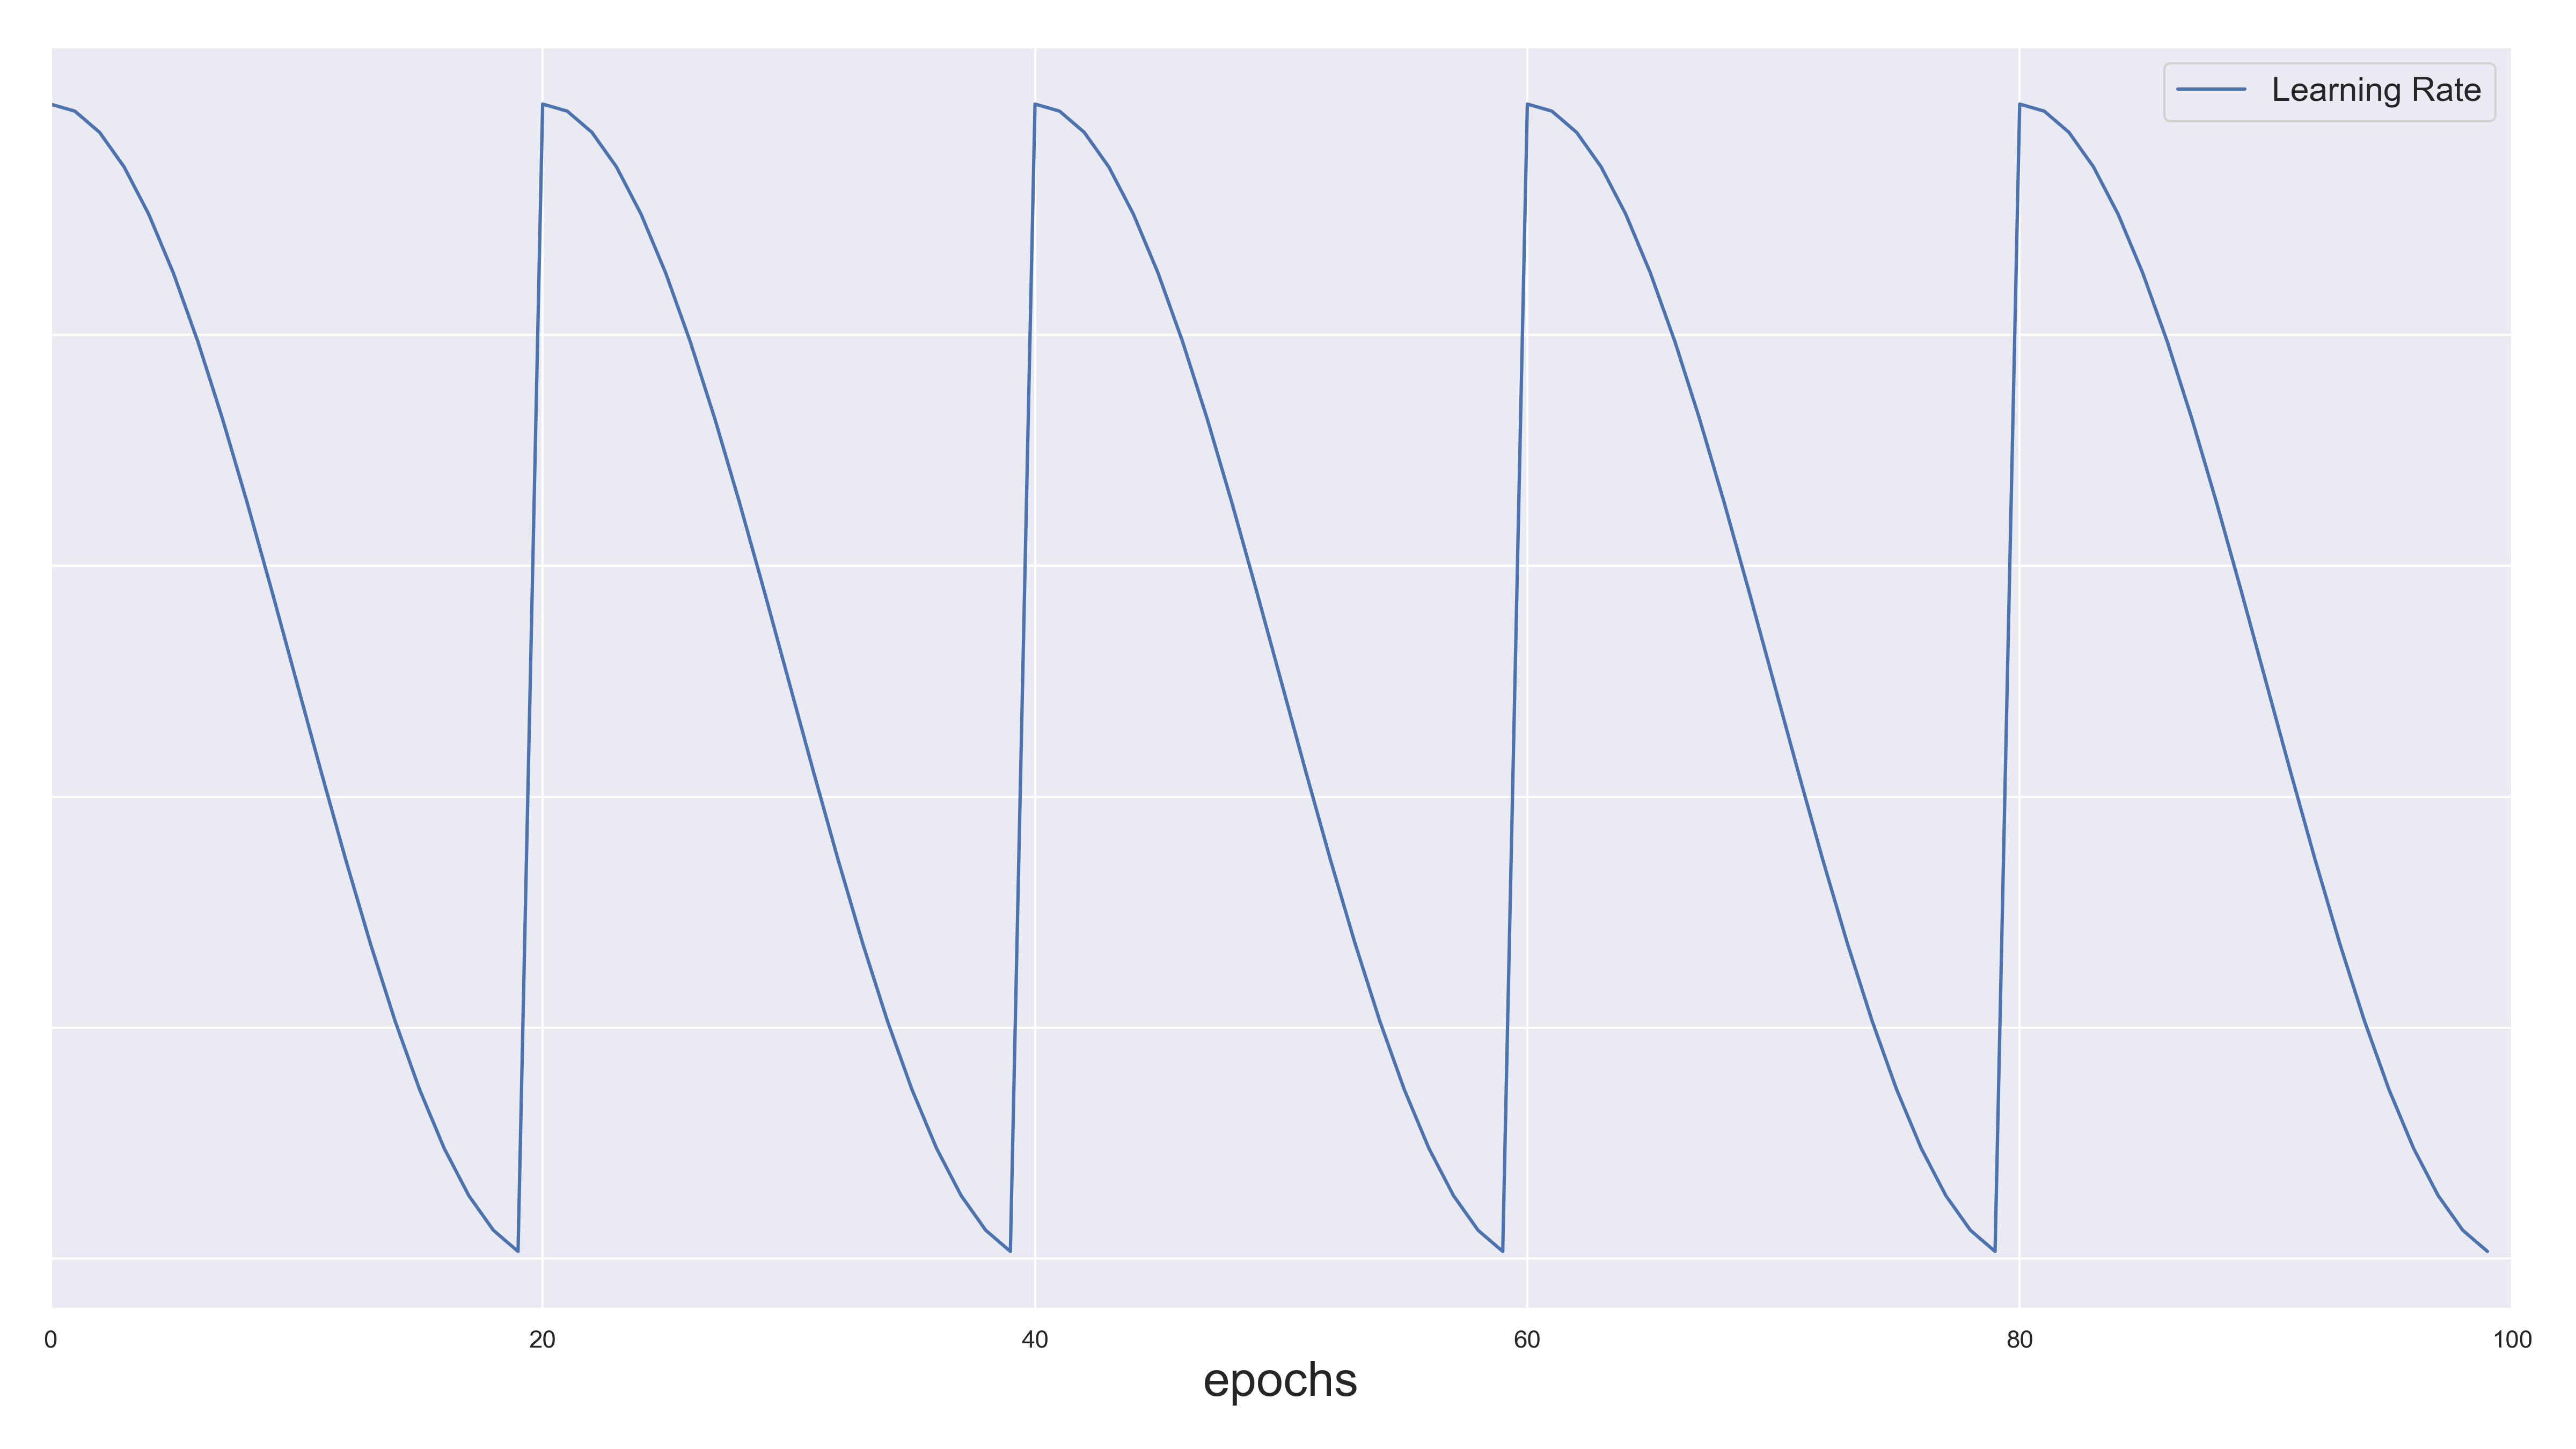
\includegraphics[width=.7\linewidth]{figures/lr.png}
		\caption[Cosine Annealing Learning Rate]{Cosine Annealing Learning Rate} \label{fig:cosineannealing}
	\end{figure}

	\item[Batch Size] Batch Size are recommend to be between 1 and a few hundreds \cite{bengio_practical_2012}, to better utilize \gls{gpu}s a batch size in the power of 2 gives better runtime, e.g. 32 to 256 \cite{goodfellow_deep_2016}. Larger batch sizes have been driving by advancements in parallelism \cite{dean_large_2012}, which can improve the training time, however smaller batch size, have shown better generalization performance due to a regularizing effect \cite{masters_revisiting_nodate}, which especially large model, that tends to overfit can benefit from \cite{goodfellow_deep_2016}. 
	
	In this project a single \gls{gpu} GTX1080 with 8Gb memory is used to train the models. A batch size of 16 is chosen for all \gls{dnn} training sessions, which is the maximum power of 2 possible with the computational budget, as the typical choice of 32 samples in a batch caused memory exhaustion. A batch size of 16 should be adequate and still provide decent training times.
	
	\item[Datasets] \gls{min100} is a subset of the \gls{ilsvrc2012} dataset \cite{russakovsky_imagenet_2015} created for this project, to reduce training time from several weeks to only days on available hardware. The sub-setting is inspired by MiniImageNet \cite{vinyals_matching_2016}, that uses a subset of 100 classes with 600 samples for each class. \gls{min100} contains 100 out of 1.000 randomly sampled classes, which gives 127.300 out of 1.2m training samples and 5.000 out of 50.000 validation samples. A full list of classes are found in the appendix. 
	
	Compared to other sufficiently dense classification datasets e.g \gls{tinyimagenet} \cite{li_cs231n:_2018}, \gls{cifar10} and \gls{cifar100} \cite{krizhevsky_cifar-10_nodate}, the image sizes of these datasets are respectively $(64\times 64$), $(32\times 32)$, $(32\times 32)$ pixels, all of which are considered too small  for this project. Other datasets such as MS COCO and Pascal VOC are better suited for object detection/segmentation, as images are not cropped to only focus on a single object, thus too challenging for classification. In fact Pascal VOC was initially tested, the model however, clearly overfitted the training data due to data sparsity. 
	
	\item[Image Augmentation] A models ability generalize a specific classification problem has a close connection with the number of available training samples. Data augmentation haven proven to be powerful tool in order to virtually create more training data \cite{perez_effectiveness_2017}. Enlarging a training dataset by data augmentation can help create new versions of an image, that are different from but still similar to the original image, without actually having to acquire and annotate new samples \cite{goodfellow_deep_2016}.  
	
	\begin{figure}[H]
		\centering
		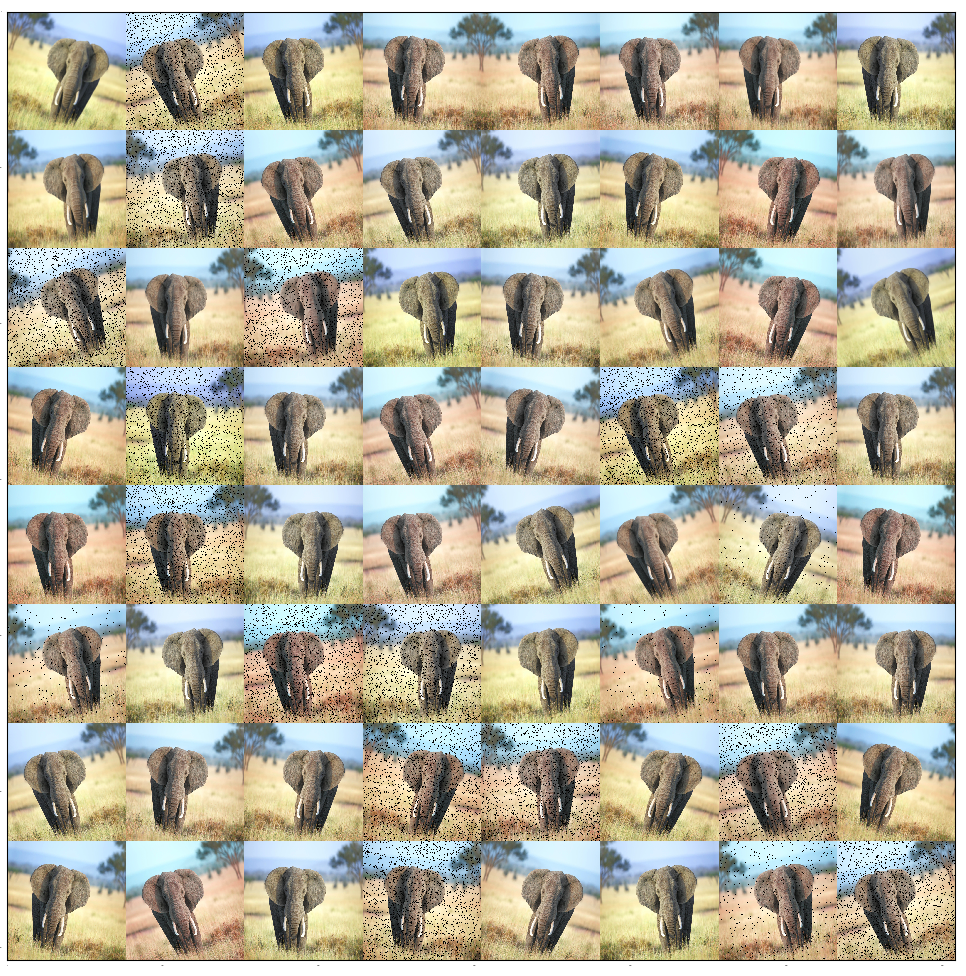
\includegraphics[width=.7\linewidth]{figures/augmentation/augmentation_high_resolution.png}
		\caption[Image Augmentaion Example]{Image Augmentation of an elephant}
		\label{fig:augmentation}
	\end{figure}
	
	Image augmentation involves transformations using tools from image processing to randomly apply noise injection, and color space transformations including contrast and saturation distortions, as well as geometric transformations, such as simple transformations of flipping the image to more complex affine transformations to create different image perspectives \cite{shorten_survey_2019}. Figure \ref{fig:augmentation} shows 64 random augmentations of an image of an elephant, achieved using \gls{imgaug} \cite{jung_imgaug:_nodate}. 
	
	New methods have been proposed where image transformations are learned to improve generalization e.g. AutoAugment \cite{cubuk_autoaugment:_2018}. 
	
	Other methods involves actually enlarging the training dataset by synthetically creating more data using a \gls{gan}. \gls{gan}s can help overcome limited data given the available training data or a 3D model, by artificially constructing new samples in different background, light setting and from alternate perspectives.
	
	Methods that do not cover enriching the available training, but alters the learning procedure are called regularization and covers; weight decay, dropout, batch normalization etc.
	
	\item[Transfer Learning] Transfer learning is the procedure of using a pre-trained model to train on a new dataset. Under the assumption, that features learned on one image dataset can be reused for another dataset \cite{yosinski_how_2014}. Transfer learning can reduce the needed time to learn general features and possibly learn better ones. Typically models have been pre-trained on the ImageNet dataset. The density of the dataset, enables model to learn general features suitable for many other domains \cite{kornblith_better_2019}. Transfer learning are especially suited for when the new data domain is of limited quantity and when the similarities between the two data domains are strong. If the similarity is less strong a model can be partially trained, the shallow layers containing general features are frozen and only the deeper layers with more specialized features are fine-tuned for the new data domain \cite{li_cs231n:_2018}.
\end{description}

\subsection{Results}

%\begin{figure}
%	\centering
%	\captionsetup[subfigure]{justification=centering}
%	\subfloat[Train loss\label{fig:B-resnet-miniimagenet10-train-loss}]{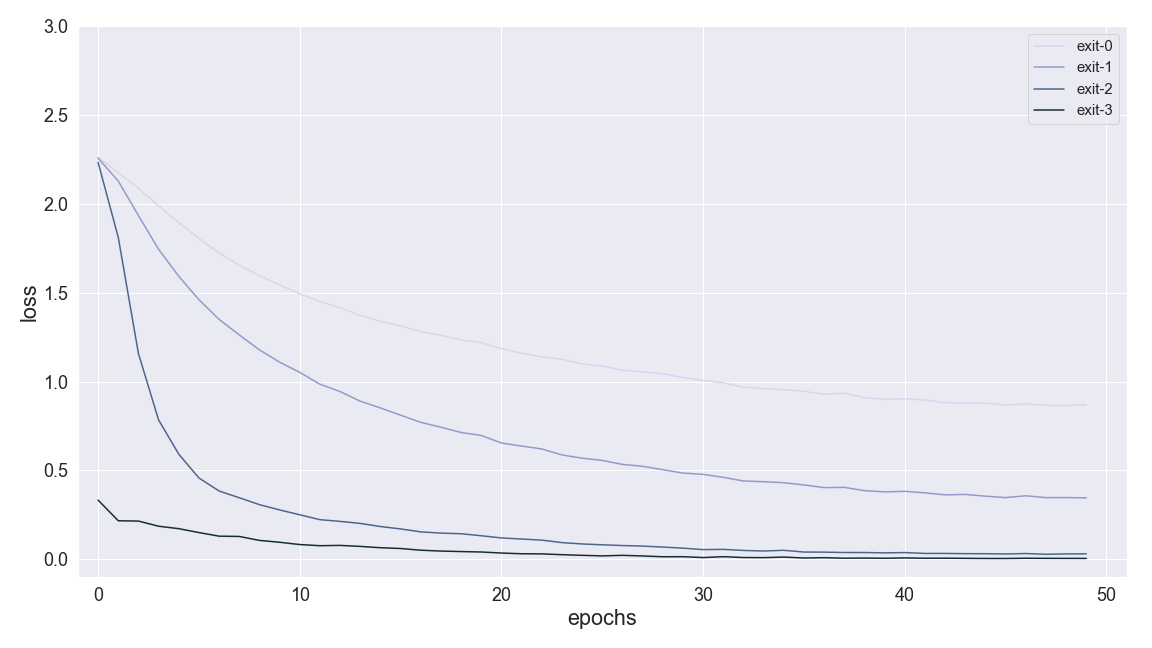
\includegraphics[width=.49\textwidth]{figures/bresnet_mini10/BResNet_train_loss_miniimagenet10.png}}
%	\subfloat[Test loss \label{fig:B-resnet-miniimagenet10-test-loss}]{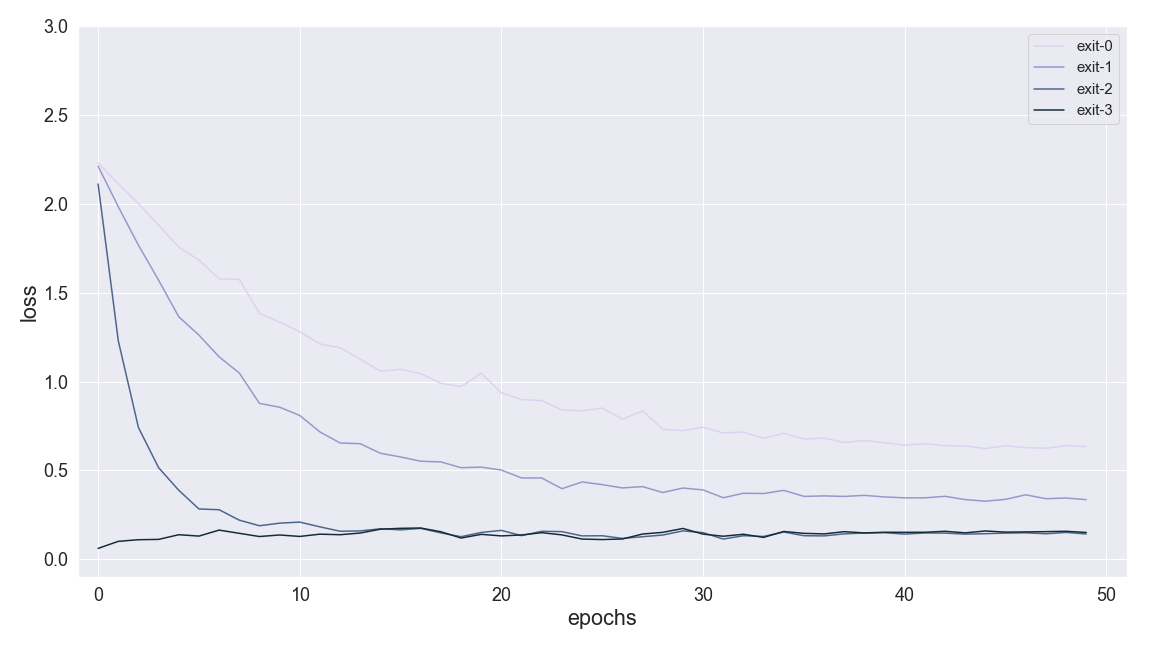
\includegraphics[width=.49\textwidth]{figures/bresnet_mini10/BResNet_test_loss_miniimagenet10.png}}
%	\hfill
%	\subfloat[Train accuracy\label{fig:B-resnet-miniimagenet10-train-acc}]{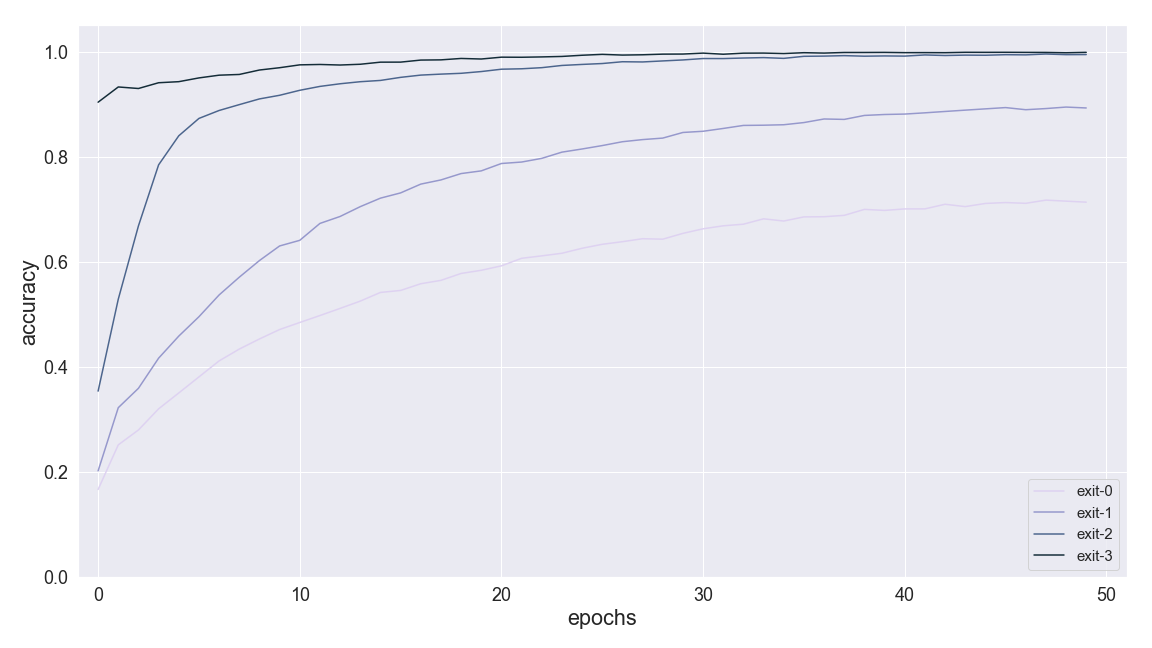
\includegraphics[width=.49\textwidth]{figures/bresnet_mini10/BResNet_train_acc_miniimagenet10.png}}
%	\subfloat[Test accuracy\label{fig:B-resnet-miniimagenet10-test-acc}]{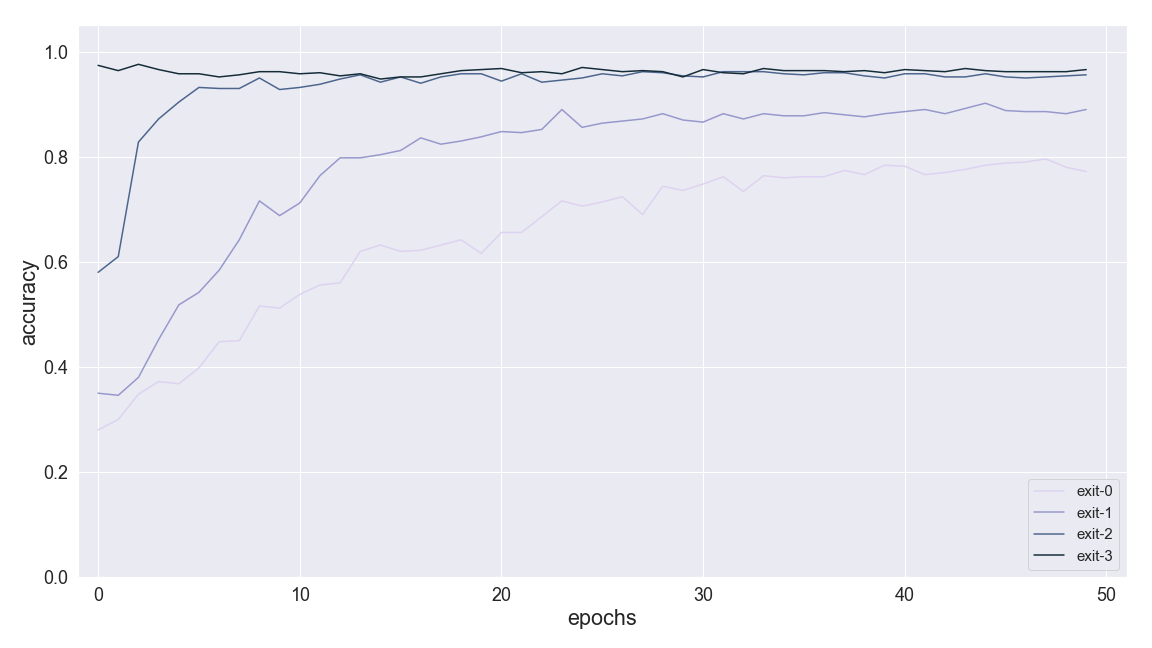
\includegraphics[width=.49\textwidth]{figures/bresnet_mini10/BResNet_test_acc_miniimagenet10.png}}
%	\caption[B-ResNet MiniImageNet10 Training summary]{Training summary shows the progression of model attributes over times of epochs, \protect\subref{fig:B-resnet-miniimagenet10-train-loss} train loss, \protect\subref{fig:B-resnet-miniimagenet10-test-loss} test loss, \protect\subref{fig:B-resnet-miniimagenet10-train-acc} train accuracy, \protect\subref{fig:B-resnet-miniimagenet10-test-acc}, test accuracy.}
%	\label{fig:B-resnet-miniimagenet-10}
%\end{figure}

Training B-\gls{resnet} and B-\gls{densenet} shows the importance of the densely connected layers for an early exiting model. The early exits of B-\gls{densenet} have a higher accuracy compared to B-\gls{resnet}, however B-\gls{resnet} last two exits are more accurate, see figure \ref{fig:b-net-miniimagenet-100}. 

\begin{figure}
	\centering
	\captionsetup[subfigure]{justification=centering}
	\subfloat[B-Resnet\label{fig:B-resnet-miniimagenet100}]{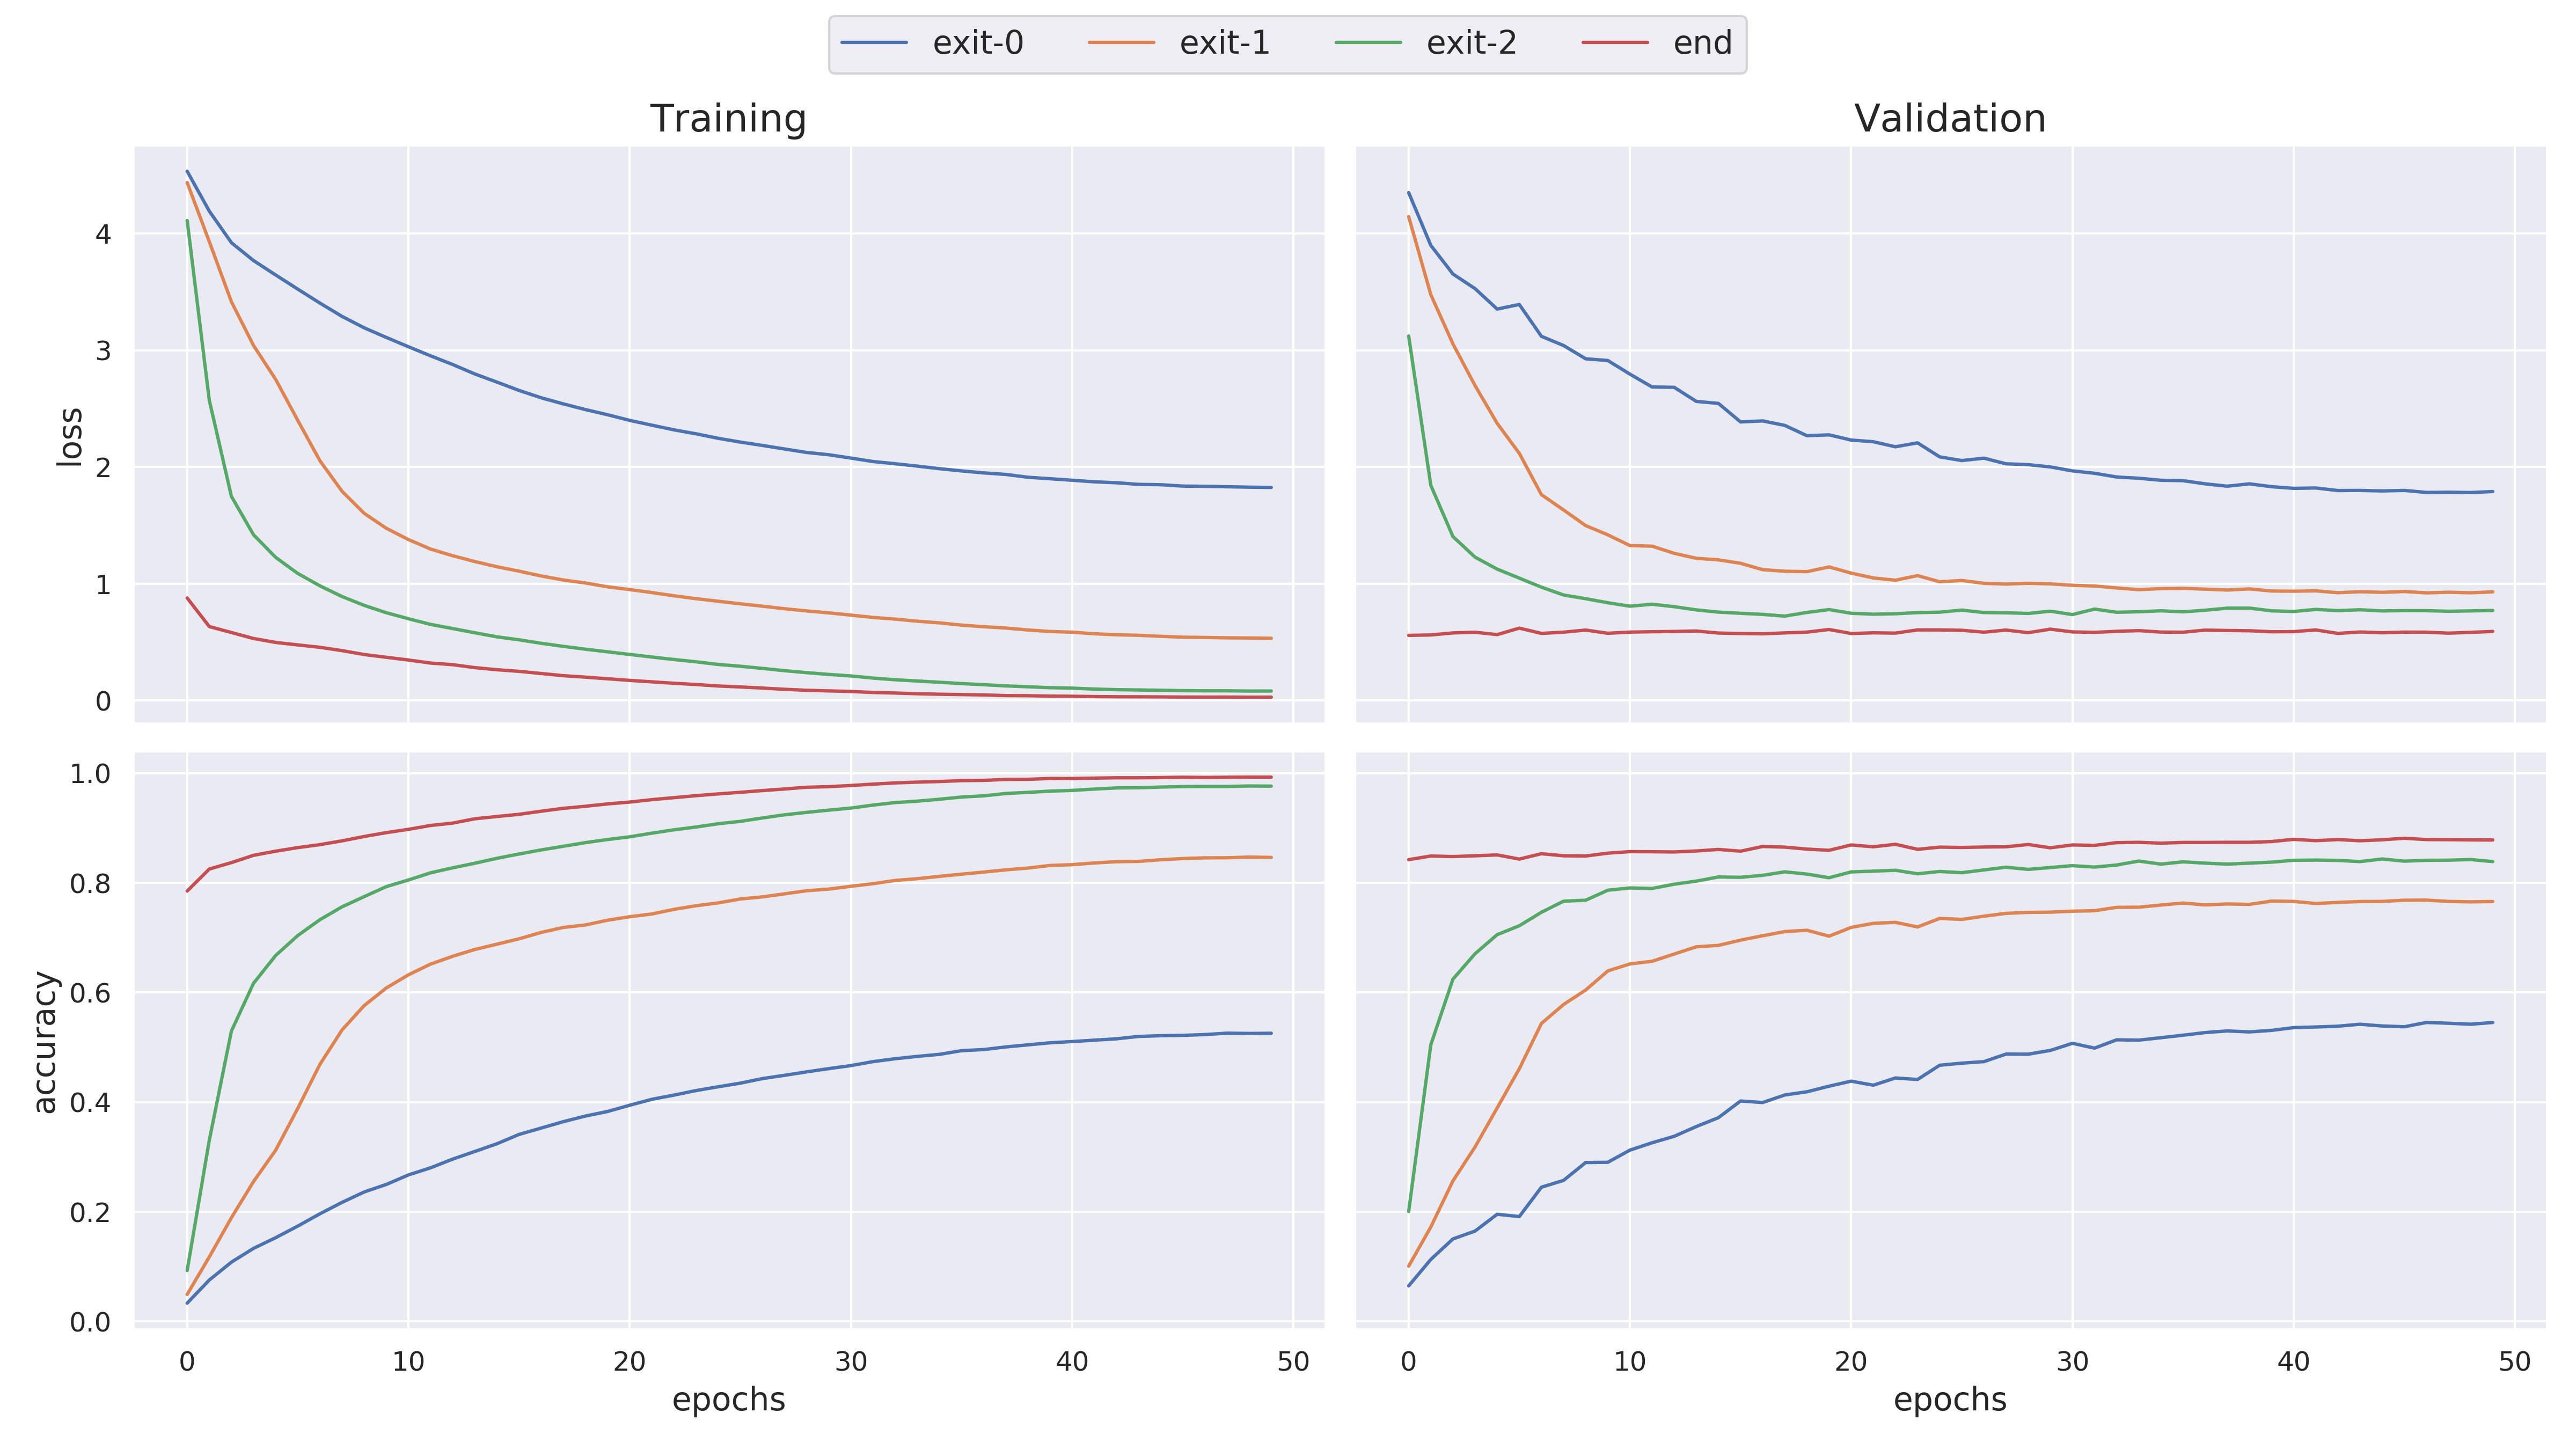
\includegraphics[width=\linewidth]{figures/training_plots/resnet_miniimagenet100}}
\end{figure}

The two last exits of \gls{resnet} are almost equally accurate. The resolution block of exit-2 are very deep, and the features becomes optimized for this classifier, hence not much gain in accuracy is obtained by running the early exit model all the way to the end. \gls{densenet} on the other hand always have an accuracy gain by continuing the inference process.    

\begin{figure}
	%\ContinuedFloat
	\captionsetup[subfigure]{justification=centering}
	\subfloat[B-DenseNet\label{fig:B-densenet-miniimagenet100}]{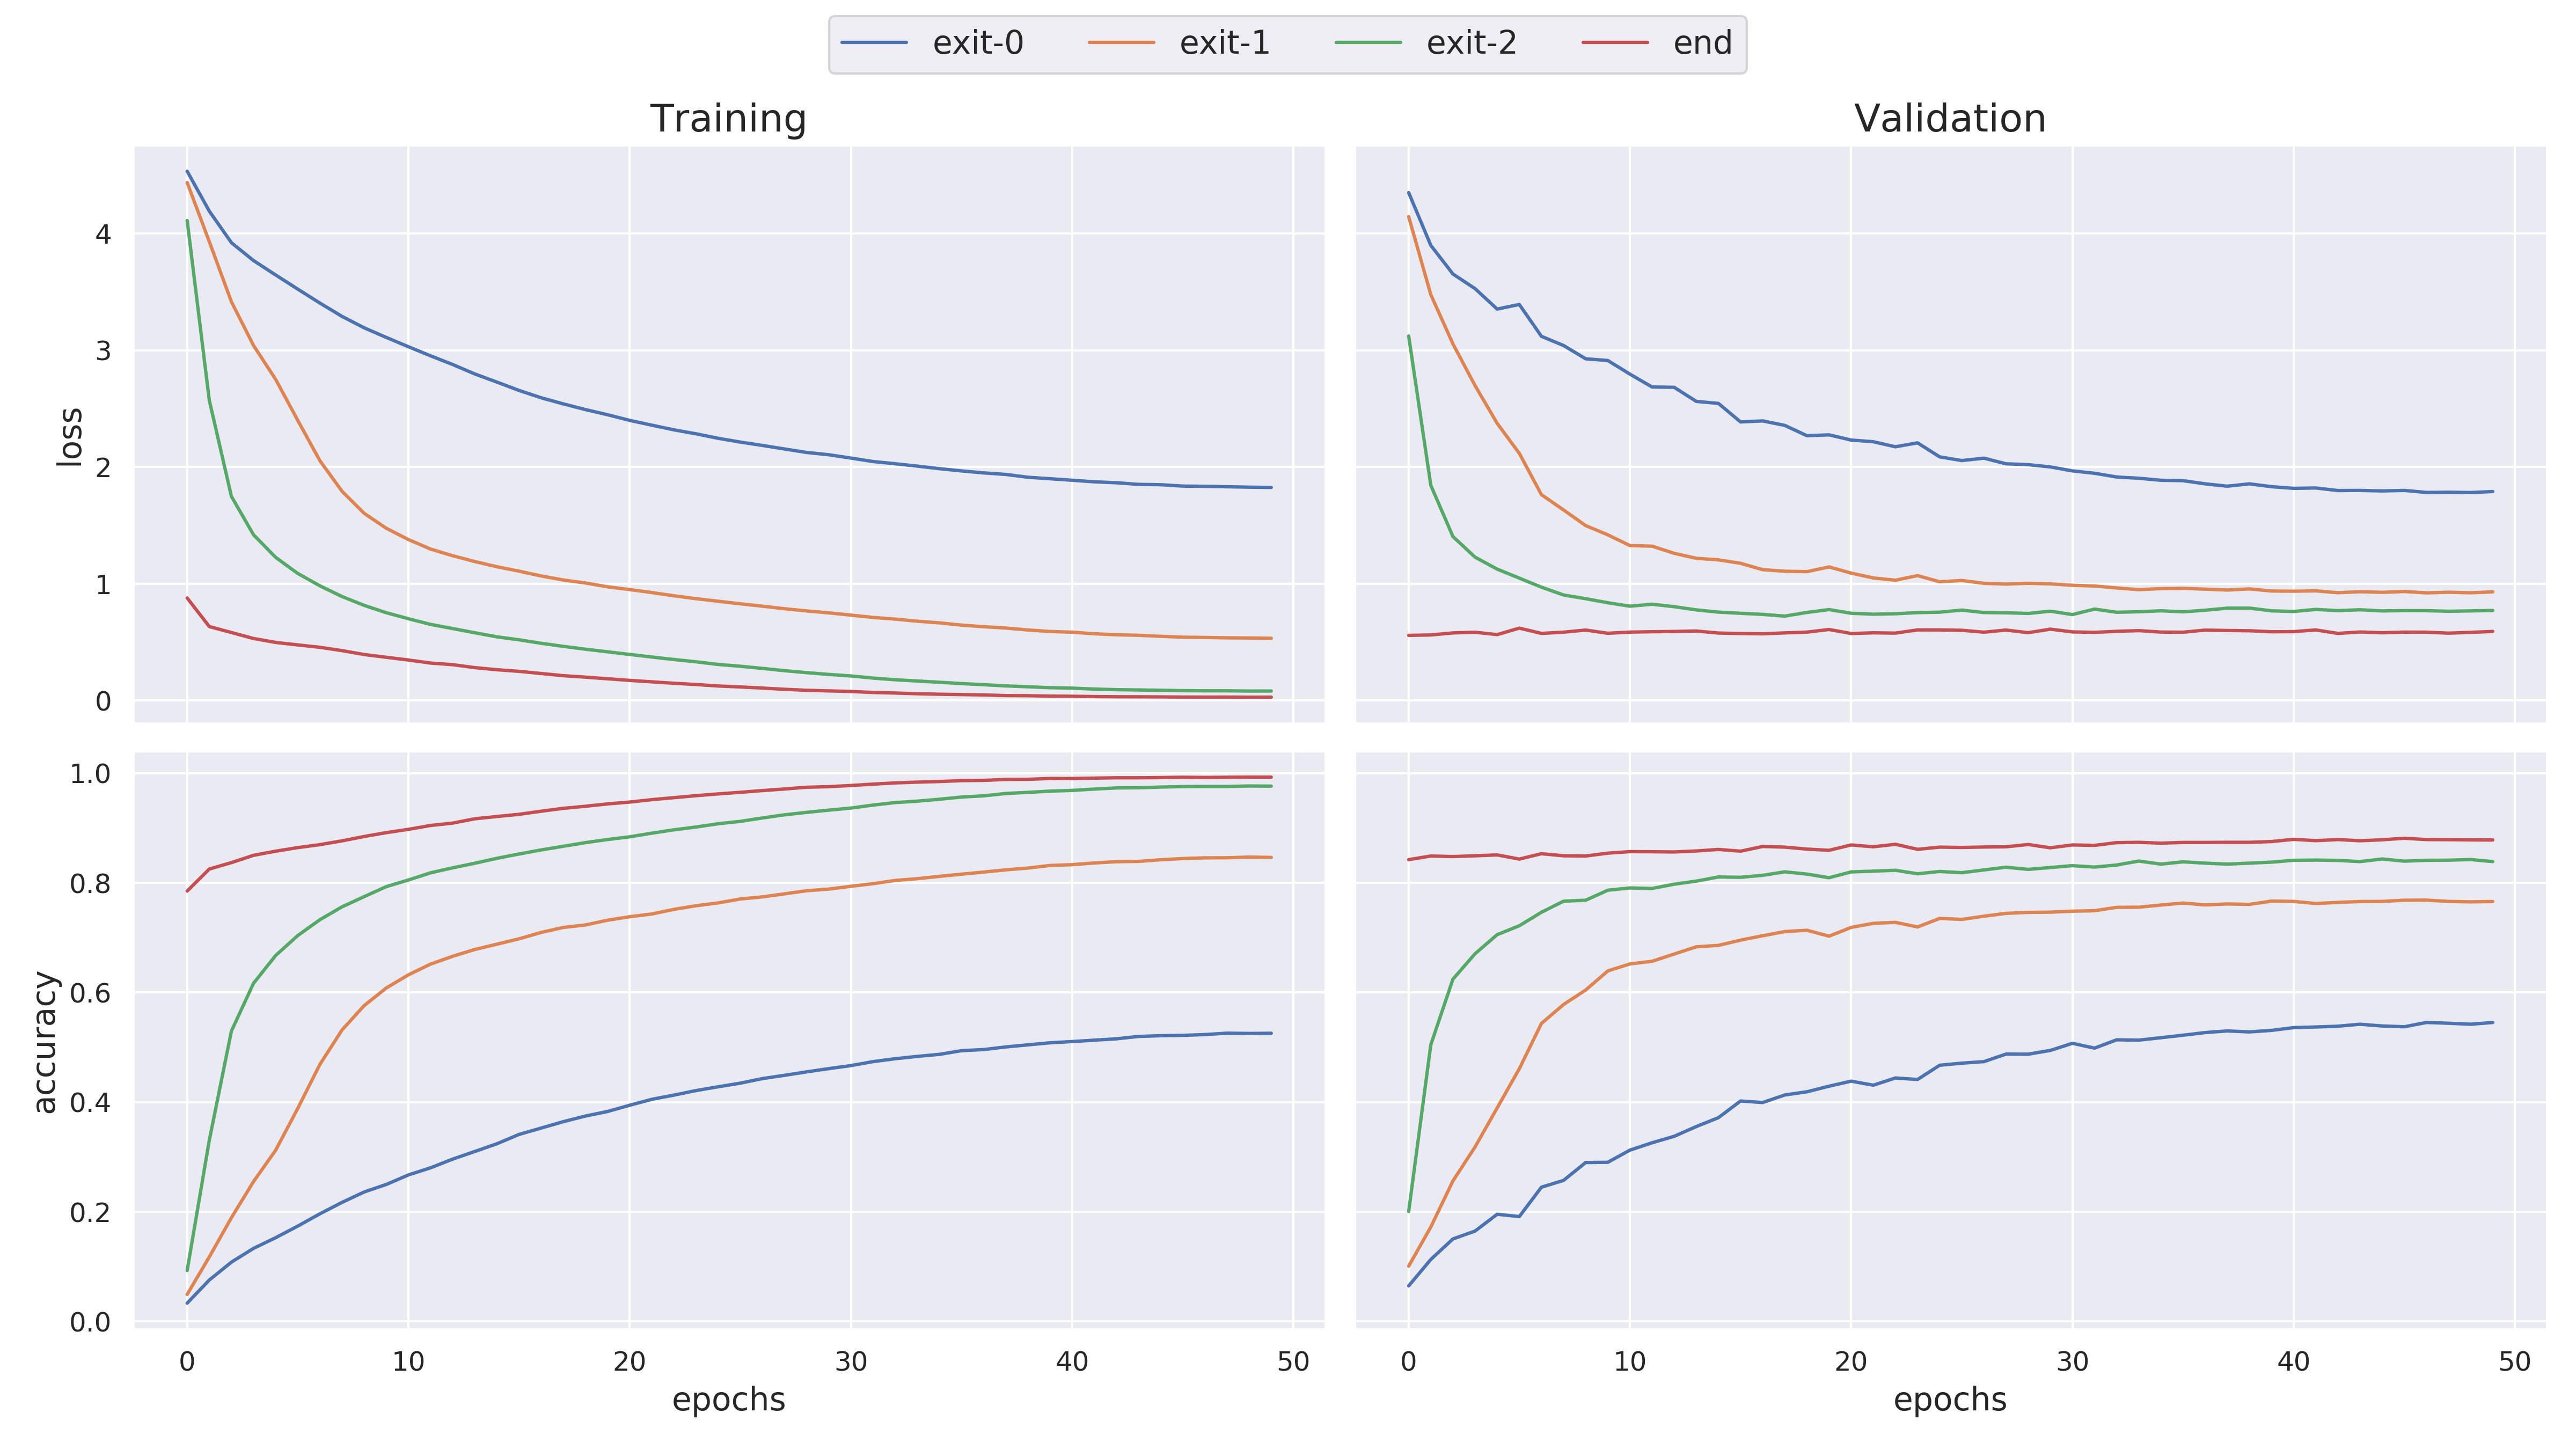
\includegraphics[width=\linewidth]{figures/training_plots/densenet_miniimagenet100}}
\end{figure}

\begin{figure}
	%\ContinuedFloat
	\captionsetup[subfigure]{justification=centering}
	\subfloat[MSDNet\label{fig:msdnet-miniimagenet100}]{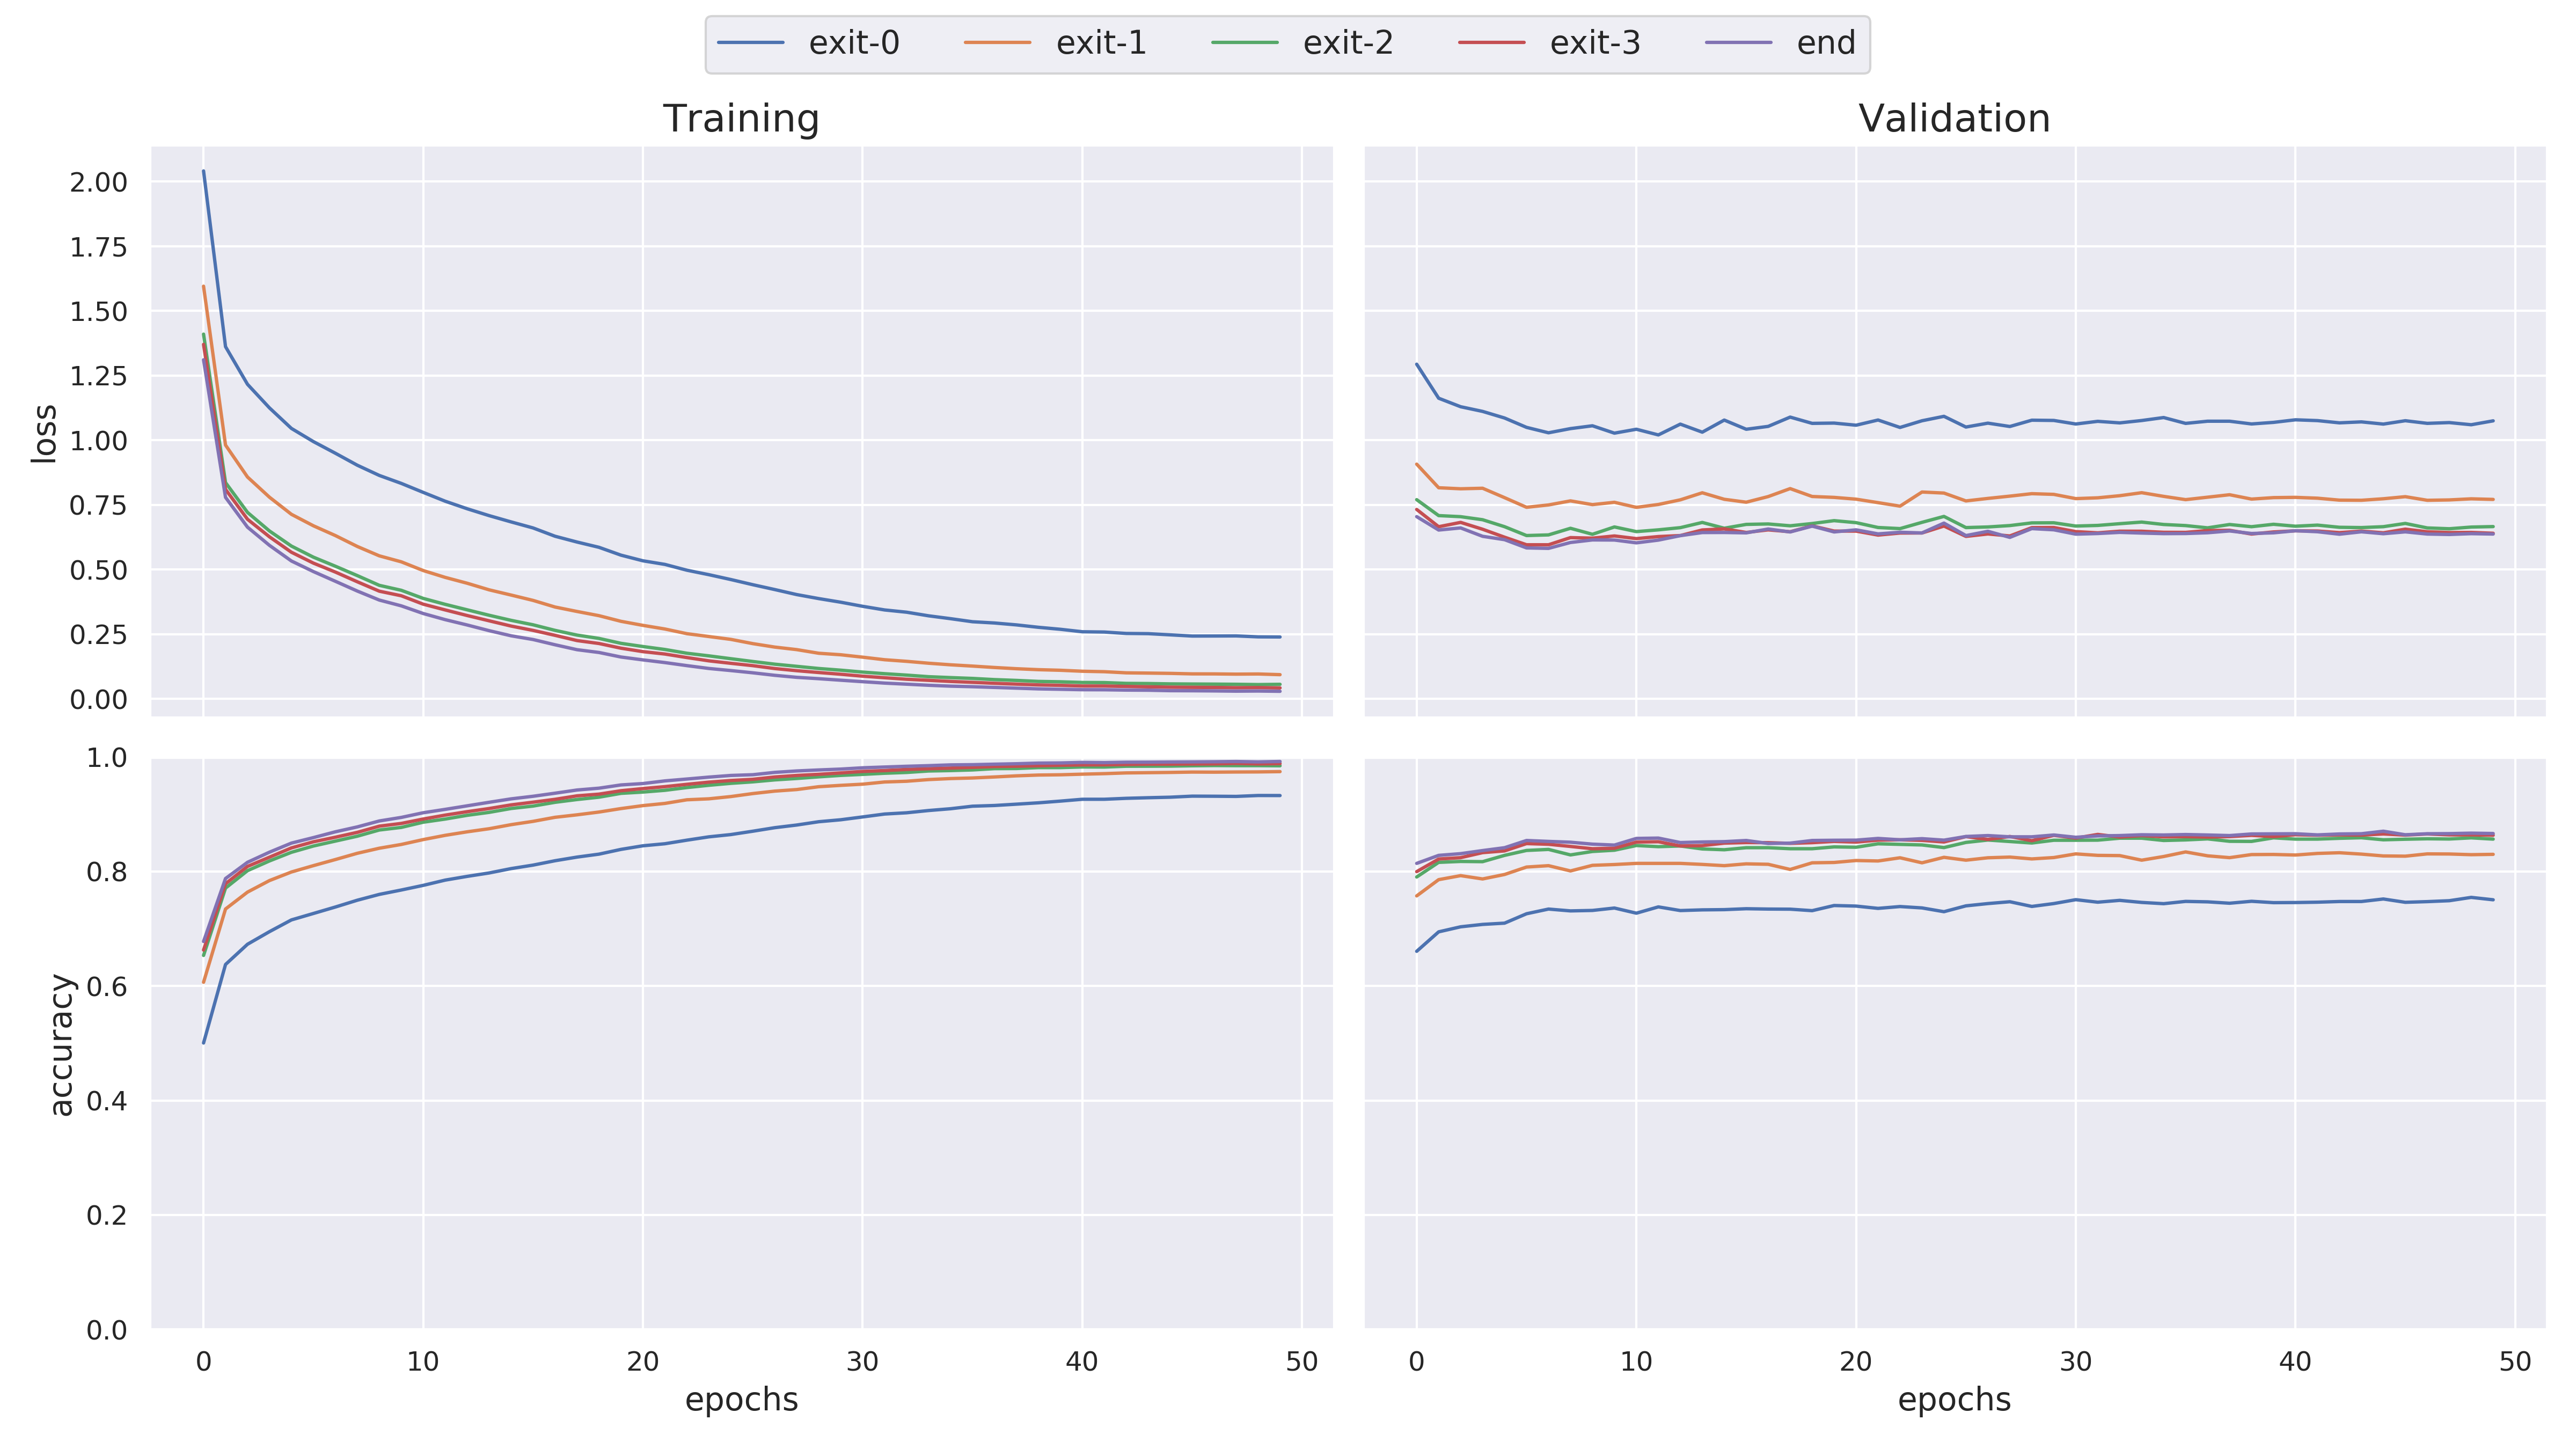
\includegraphics[width=\linewidth]{figures/training_plots/msd_miniimagenet100}}
	\caption[Training progress of BrancyNets]{Training progress for \protect\subref{fig:B-resnet-miniimagenet100} B-ResNet, \protect\subref{fig:B-densenet-miniimagenet100} B-DenseNet and \protect\subref{fig:msdnet-miniimagenet100} MSDNet} 
	\label{fig:b-net-miniimagenet-100}
\end{figure}

\subsection{Validation}

In this test all validation samples are inferred to all three models. Each branch classifies the samples, but does not perform exit but continues the inference process. Figure \ref{fig:exit-accuracy} show the accuracy of each exit.  

\begin{figure}
	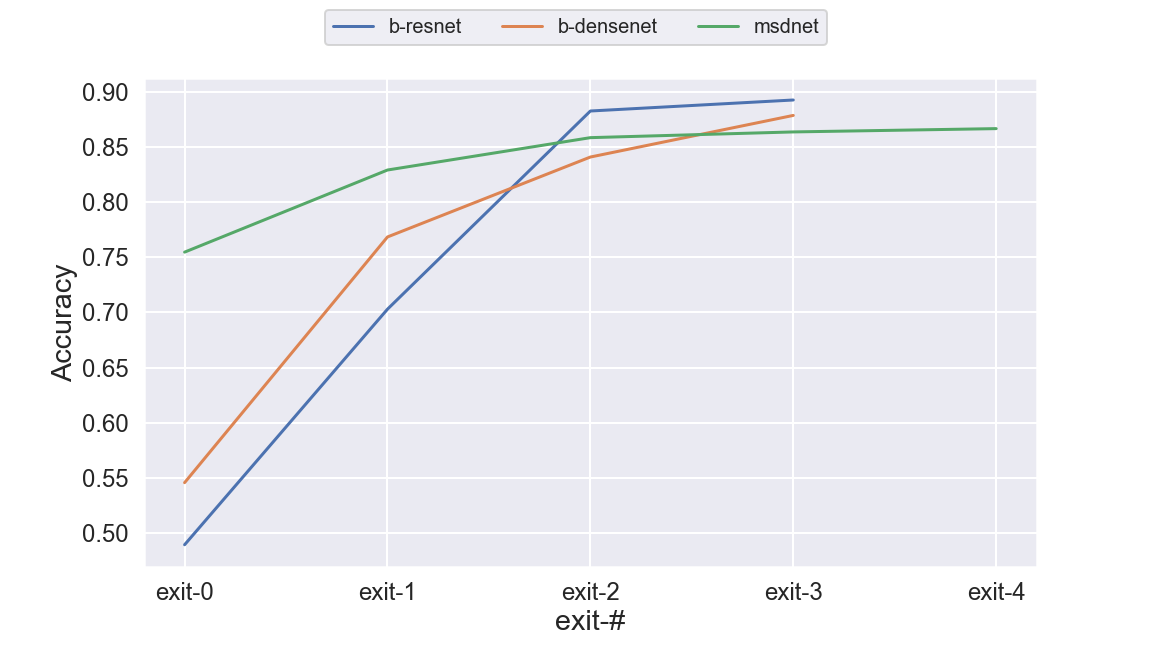
\includegraphics[width=\linewidth]{figures/inference_plots/exit_acc}
	\caption[Model Inference Accuracy]{Model Inference Accuracy}
	\label{fig:exit-accuracy}
\end{figure}

As expected the models become more accurate as we go deeper in the network. The features deep within the network have more discriminative characteristics. As stated in \cite{huang_multi-scale_2017} the densely connected features are important factors for obtaining intermediate classifiers with decent accuracy. The B-\gls{densenet} and \gls{msdnet} have as expected more accurate early classifiers, however the end-exit of B-\gls{resnet} achieves superior accuracy compared to the other models.

Still about half the samples can be accurately classified at the very first exit, which justifies the assumption for \gls{branchynet} and we can expectedly save time but let samples exit prematurely,


\section{Early Exiting Analysis}

\subsection{Experimental Setup}




\begin{longtabu}{>{\bfseries}X[0.8]|X[0.8]|X[1.5]|X[r0.3]}
	\caption[Platform hardware comparison]{Platform hardware comparison of Window 10 Stationary PC and NVIDIA Jetson TX2 Edge Computer} \label{tbl:platforms} \\
	\toprule
	\rowfont{\bfseries}
	Platform & CPU & GPU & RAM  \tabularnewline
	\bottomrule
	\endfirsthead
	\multicolumn{3}{@{}l}{\textbf{\textcolor{black}{Table \ref{tbl:platforms}:}} continued}\\
	\toprule
	\rowfont{\bfseries}
	Platform & CPU & GPU & RAM  \tabularnewline
	\bottomrule
	\endhead % all the lines above this will be repeated on every page
	\bottomrule
	\multicolumn{3}{@{}l}{continued \ldots}\\
	\endfoot
	\hline
	\endlastfoot
	Windows PC	& Intel i5-6600K.	& NVIDIA GeForce GTX 1080, 2560 CUDA cores	& 16GB \tabularnewline
	\hline
	Jetson TX2	& ARM Cortex-A57 	& NVIDIA Pascal GPU, 256 CUDA cores 		& 8GB \tabularnewline
	\hline
	NUC		  	& Intel i7-7567U	& None										& 16GB \tabularnewline									
	\bottomrule
\end{longtabu}

\subsection{Accuracy-Latency Analysis}

 see figure \ref{fig:exit-time}

\begin{figure}
	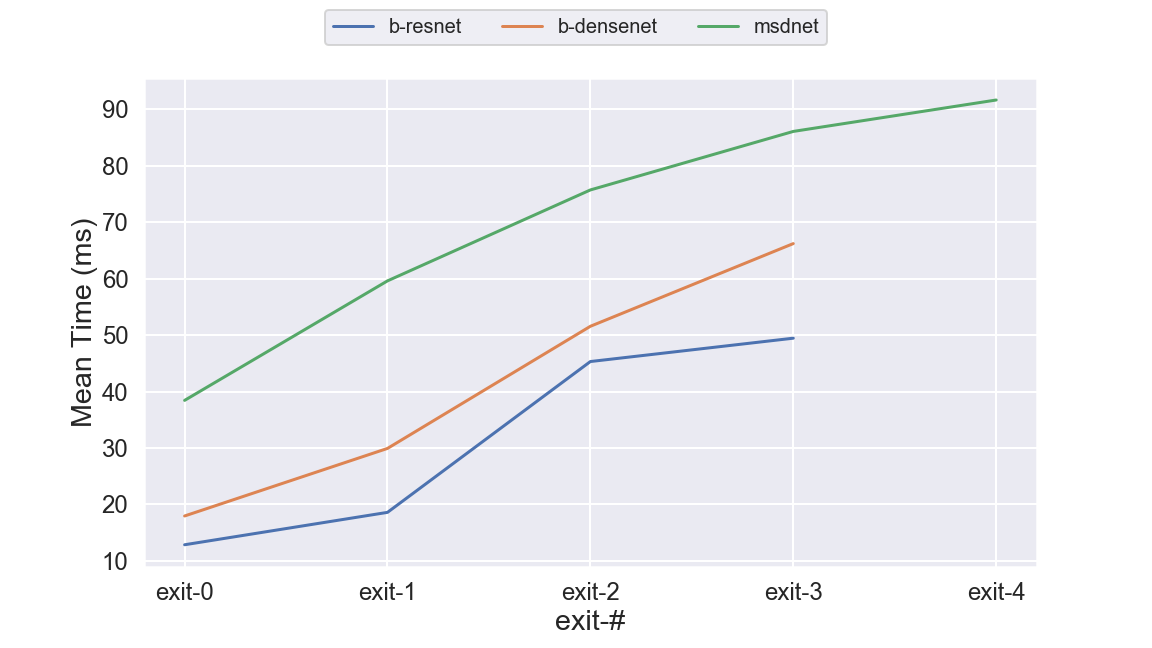
\includegraphics[width=\linewidth]{figures/inference_plots/exit_time}
	\caption[Model Inference Accuracy]{Model Inference Time}
	\label{fig:exit-time}
\end{figure}



Figure \ref{fig:exit-time} shows the average inference time for a classification at the corresponding exit. If the model decides to exit earlier in the network, the figure shows the time savings achievable. The inference time is hardware dependent and a full model comparison cannot be made solely by this test, later tests compares the inference time of the models on different platforms, however the trend seems to be, that B-\gls{resnet} is the fastest, followed by B-\gls{densenet} an lastly \gls{msdnet}. Table \ref{tbl:early-exit} shows the accuracy and mean time in tabular form.

\begin{longtabu}{>{\bfseries}X|X[r]|X[r]|X[r]|X[r]|X[r]}
	\caption[Early exit models' last exit accuracy]{Early exit models' last exit accuracy. Model Parametric Comparison using \texttt{thop} \cite{zhu_thop_nodate}. The test is conducted by inference a random 4d tensor of size $ (\mathrm{batch,channels,width,height})=(1,3,224,224) $ to all models.}\label{tbl:early-exit} \\
	\toprule
	\rowfont{\bfseries}
	Model & Accuracy & Mean Time (ms) & Layers & Parameters (M) & G\gls{flop}s \tabularnewline
	\hline
	\endfirsthead
	\multicolumn{3}{@{}l}{\textbf{\textcolor{black}{Table \ref{tbl:early-exit}:}} continued}\\
	\toprule
	\rowfont{\bfseries}
	Model & Accuracy & Mean Time (ms) & Layers & Parameters (M) & G\gls{flop}s \tabularnewline
	\hline
	\endhead % all the lines above this will be repeated on every page
	\hline
	\multicolumn{3}{@{}l}{continued \ldots}\\
	\endfoot
	\hline
	\endlastfoot
	ResNet  &  & & $ 101 $ & $ 42.705 $ & $ 7.864 $ \tabularnewline
	\hline
	DenseNet & & & $ 121 $ & $ 7.056 $ & $ 2.897 $ \tabularnewline
	\hline
	B-ResNet & & & $ 107 $ & $ 42.885 $ & $ 7.866 $ \tabularnewline 
	\hspace{3mm} Exit-0 & 0.489 & 12.87 & & & \tabularnewline
	\hspace{3mm} Exit-1 & 0.703 & 18.61 & & &\tabularnewline
	\hspace{3mm} Exit-2 & 0.883 & 45.31 & & &\tabularnewline
	\hspace{3mm} Exit-3 & 0.893 & 49.45 & & &\tabularnewline
	\hline
	B-DenseNet &  & & $ 127 $ & $ 7.236 $ & $ 2.898 $\tabularnewline
	\hspace{3mm} Exit-0 & 0.545 & 17.96 & & & \tabularnewline
	\hspace{3mm} Exit-1 & 0.769 & 29.93 & & &\tabularnewline
	\hspace{3mm} Exit-2 & 0.841 & 51.56 & & &\tabularnewline
	\hspace{3mm} Exit-3 & 0.879 & 66.20 & & &\tabularnewline
	\hline
	MSDNet & & & $ 24 $ & $ 23.958 $ & $ 1.374 $ \tabularnewline
	\hspace{3mm} Exit-0 & 0.755 & 38.43 & & &\tabularnewline
	\hspace{3mm} Exit-1 & 0.829 & 59.60 & & &\tabularnewline
	\hspace{3mm} Exit-2 & 0.859 & 75.70 & & &\tabularnewline
	\hspace{3mm} Exit-3 & 0.864 & 86.06 & & &\tabularnewline
	\hspace{3mm} Exit-4 & 0.867 & 91.63 & & &\tabularnewline
	\bottomrule
\end{longtabu}


The challenge is to known when to let samples exit, which can either be done at random or using the output from the softmax function, which can be interpreted as a confidence metric for the prediction. In the next test, we evaluate the two mentioned confidence scores as a threshold for exiting. 

\begin{figure}
	\captionsetup[subfigure]{farskip=0pt,captionskip=0pt, justification=centering}
	\centering
	\subfloat{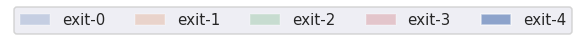
\includegraphics[width=.5\textwidth,height=\textheight,keepaspectratio]{figures/threshold_plots/time_dist_legend}}
	\hfill
	\subfloat[Windows PC]{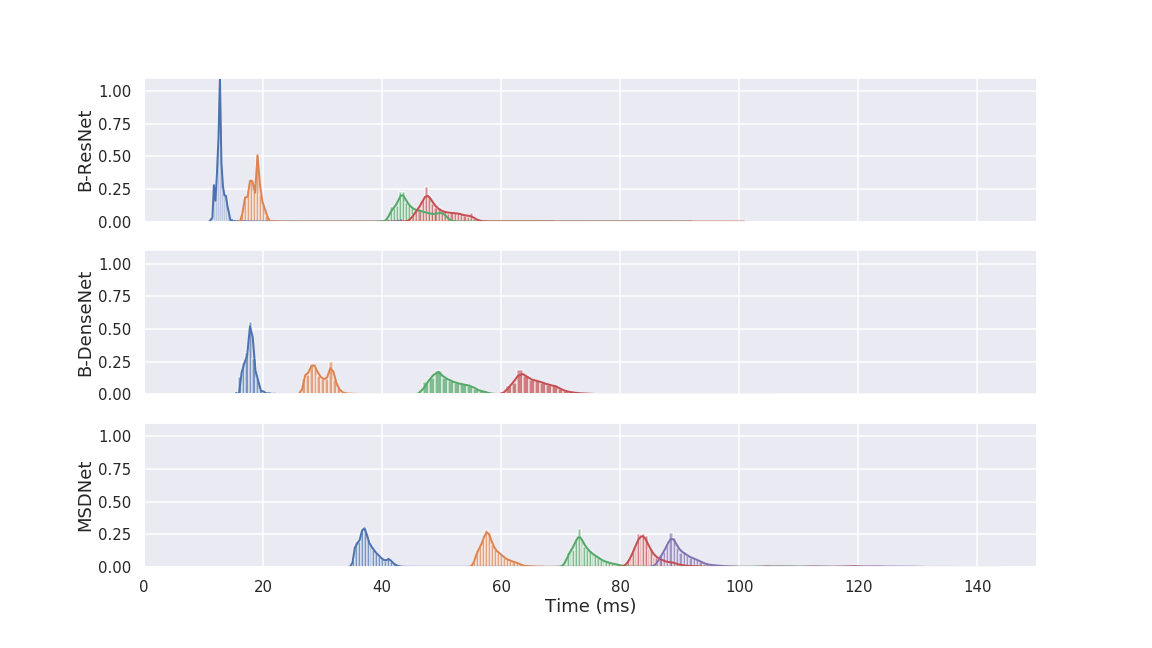
\includegraphics[width=\textwidth,height=.29\textheight,keepaspectratio]{figures/threshold_plots/inference_time_distribution}}
	\hfill
	\subfloat[Jetson TX2]{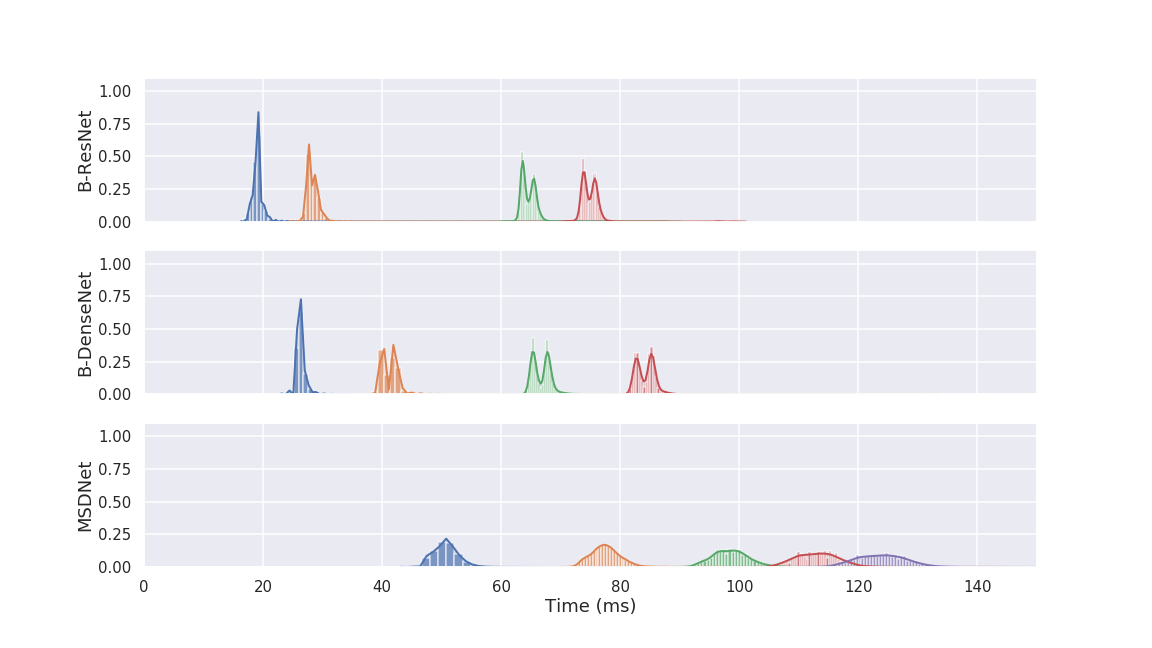
\includegraphics[width=\textwidth,height=.29\textheight,keepaspectratio]{figures/threshold_plots/jetson_inference_time_distribution}}
	\hfill
	\subfloat[NUC]{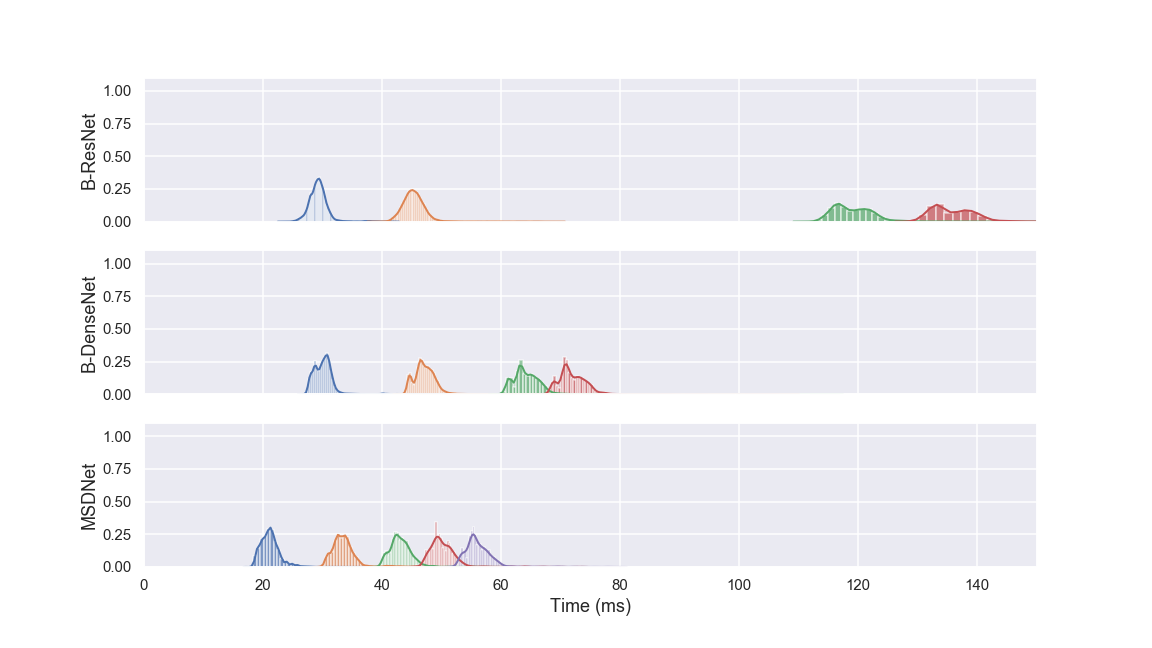
\includegraphics[width=\textwidth,height=.29\textheight,keepaspectratio]{figures/threshold_plots/nuc_inference_time_distribution}}
	\caption[Inference Time Distribution]{Inference Time Distribution}
	\label{fig:inference-time-dist}
\end{figure}


%\paragraph{Pascal VOC}
%
%\begin{figure}
%	\centering
%	\captionsetup[subfigure]{justification=centering}
%	\subfloat[Train loss\label{fig:B-resnet-voc-train-loss}]{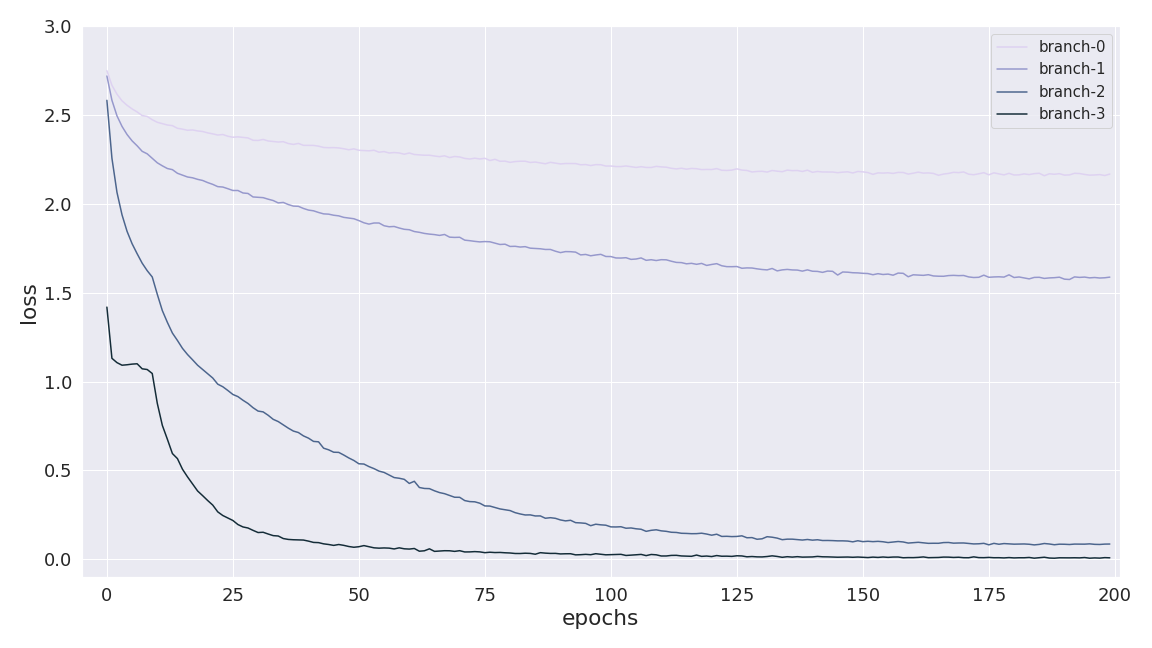
\includegraphics[width=.49\textwidth]{figures/BResNetVOC/BResNet_train_loss_VOC.png}}
%	\subfloat[Test loss \label{fig:B-resnet-voc-test-loss}]{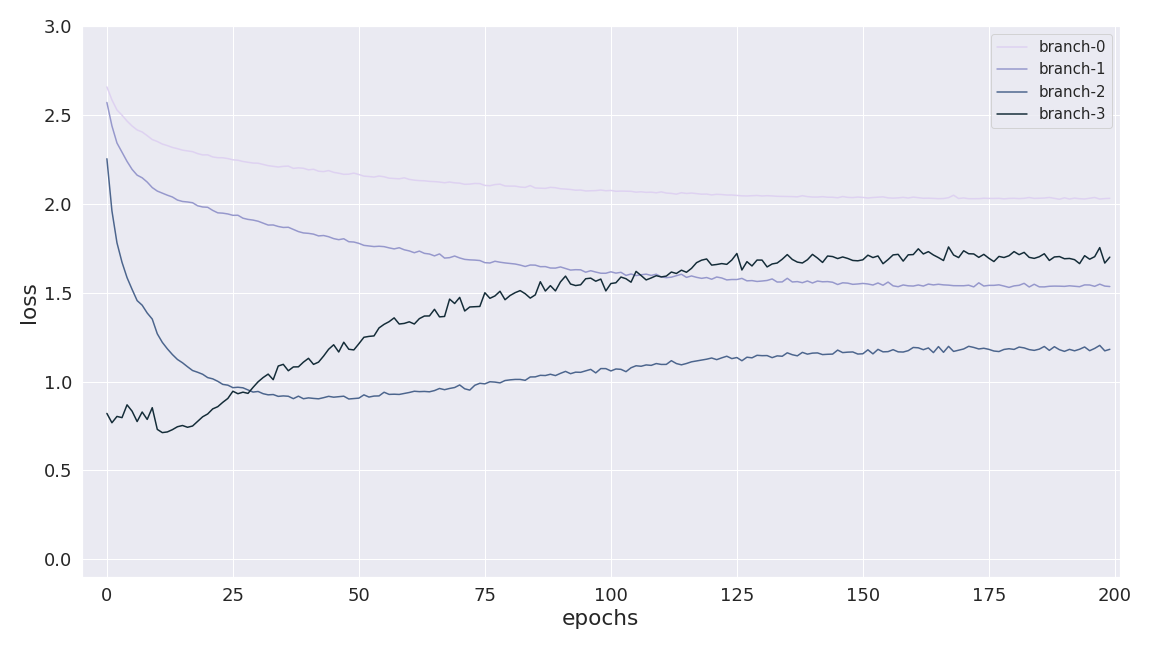
\includegraphics[width=.49\textwidth]{figures/BResNetVOC/BResNet_test_loss_VOC.png}}
%	\hfill
%	\subfloat[Train accuracy\label{fig:B-resnet-voc-train-acc}]{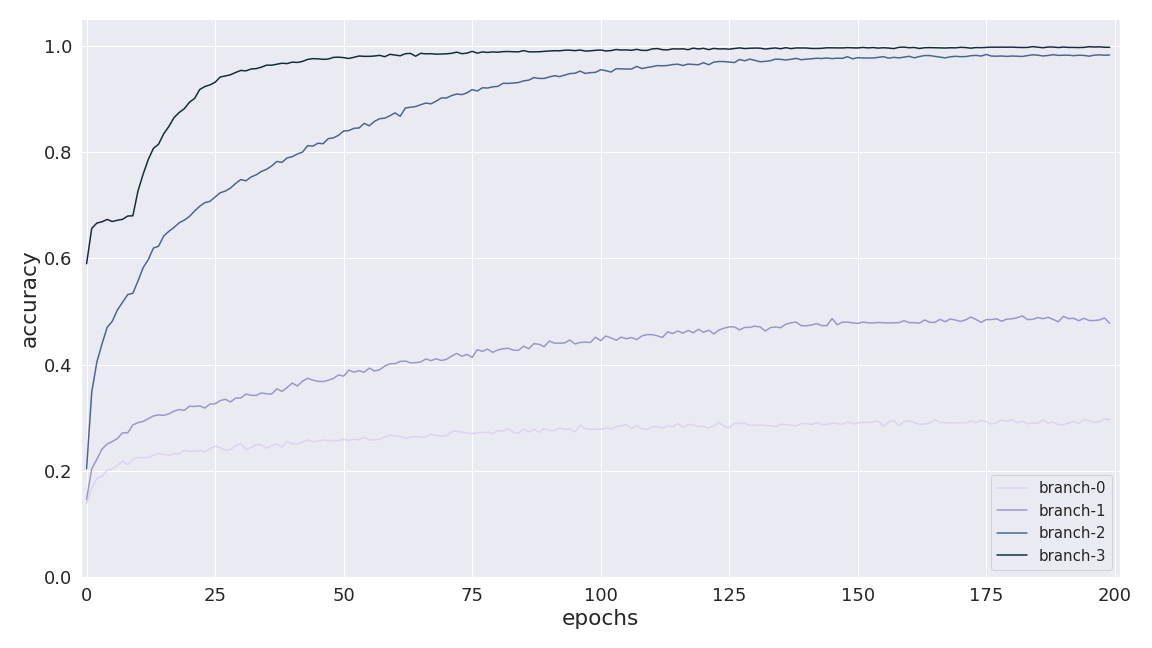
\includegraphics[width=.49\textwidth]{figures/BResNetVOC/BResNet_train_acc_VOC.png}}
%	\subfloat[Test accuracy\label{fig:B-resnet-voc-test-acc}]{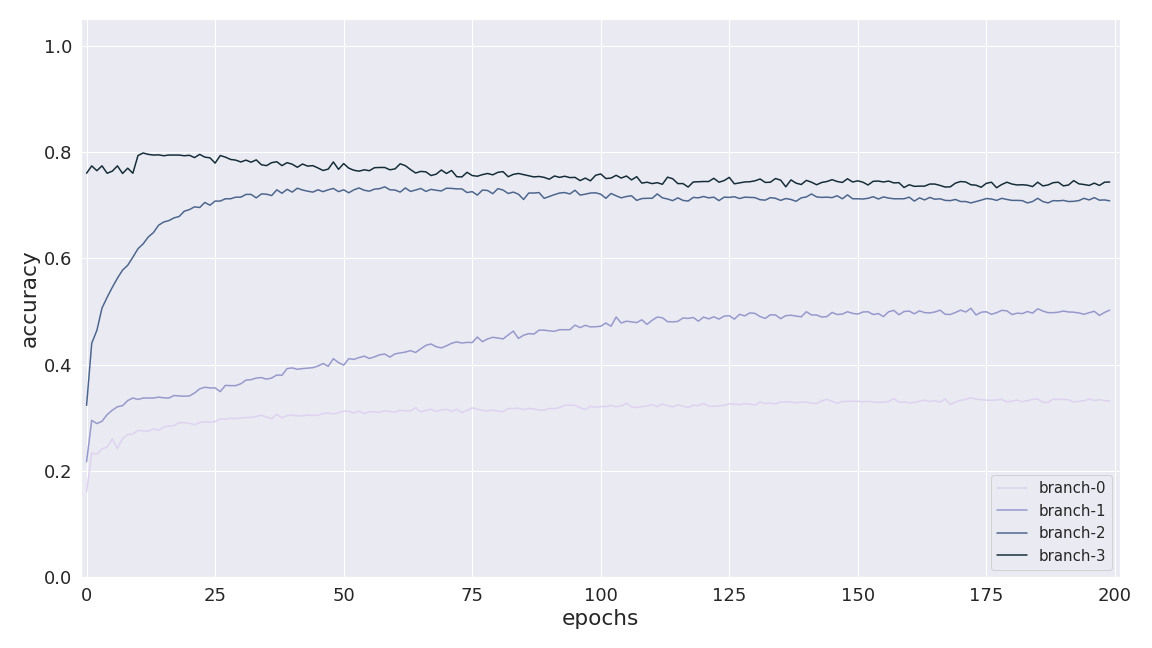
\includegraphics[width=.49\textwidth]{figures/BResNetVOC/BResNet_test_acc_VOC.png}}
%	\caption[B-ResNet VOC Training summary]{Training summary shows the progression of model attributes over times of epochs, \protect\subref{fig:B-resnet-voc-train-loss} train loss, \protect\subref{fig:B-resnet-voc-test-loss} test loss, \protect\subref{fig:B-resnet-voc-train-acc} train accuracy, \protect\subref{fig:B-resnet-voc-test-acc}, test accuracy.}
%\end{figure}
%
%Visualizing the training progression, clearly indicates that model overfitting to the training data. When a model overfits it suffers to generalize the true underlying distribution of the data. This can be caused by insufficient number of training samples or too complex a model. Since the model has shown promising results in image classification task previously, we can conclude, that the dataset is too sparse.
%
%Even though the model fails to generalize, the experiment still produce interesting results. Given an early exiting model as B-ResNet 50\% of the test samples can be correctly classified using only half of the \gls{dnn}.


\subsection{Confidence Threshold Analysis}

In this experiment the MiniImageNet100 validation set have been used to evaluate the two threshold metrics; \emph{Confidence Threshold} and \emph{Score-Margin Threshold}. \Cref{fig:resnet_confidence,fig:resnet_score-margin,fig:densenet_confidence,fig:densenet_score-margin,fig:msdnet_confidence,fig:msdnet_score-margin} compares the performance of each exit on all samples. The figures show for each of the three networks under test a plot of the two thresholds for all exit for the model. It shows the frequency of exited samples, that have been correctly classified ({\color{sns-green}green}) and incorrectly classified ({\color{sns-red}red}). As well as, samples that could not be classified with proper confidence given the threshold metric, hence not exited at the exit ({\color{sns-blue}blue}). Along with a plot of the change in accuracy for the exit as the confidence grows ({\color{sns-orange}orange}).  

\newcounter{imagenumber}
\begin{minipage}{\textwidth}
\begin{figure}
	\centering
	\paragraph{B-ResNet}
	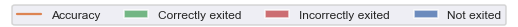
\includegraphics[width=\linewidth]{figures/threshold_plots/threshold_analysis_legend}
\end{figure}

\begin{minipage}{0.5\textwidth}
	\begin{figure}
		\captionsetup[subfloat]{farskip=1pt,captionskip=1pt, justification=centering}
		\centering
		\forloop{imagenumber}{0}{\value{imagenumber} < 4}{
			
			\subfloat[Exit-\arabic{imagenumber}\label{fig:confidence_resnet_exit_\arabic{imagenumber}}]{\includegraphics[width=.9\linewidth]{figures/threshold_plots/threshold_analysis_b-resnet_confidence_\arabic{imagenumber}}}
			\hfill
		}
		\caption[ResNet Confidence Threshold]{Confidence Threshold}
		\label{fig:resnet_confidence}
	\end{figure}
\end{minipage}
\begin{minipage}{0.5\textwidth}
	\begin{figure}
		\captionsetup[subfloat]{farskip=1pt,captionskip=1pt, justification=centering}
		\centering
		\forloop{imagenumber}{0}{\value{imagenumber} < 4}{
			
			\subfloat[Exit-\arabic{imagenumber}\label{fig:score-margin_resnet_exit_\arabic{imagenumber}}]{\includegraphics[width=.9\linewidth]{figures/threshold_plots/threshold_analysis_b-resnet_score-margin_\arabic{imagenumber}}}
			\hfill
		}
		\caption[ResNet Score-margin Threshold]{Score-margin Threshold}
		\label{fig:resnet_score-margin}
	\end{figure}
\end{minipage}
\end{minipage}

\begin{minipage}{\textwidth}
	\begin{figure}
		\centering
		\paragraph{B-DenseNet}
	\end{figure}
	\begin{minipage}{0.5\textwidth}
		\begin{figure}
			\captionsetup[subfloat]{farskip=1pt,captionskip=1pt, justification=centering}
			\centering
			\forloop{imagenumber}{0}{\value{imagenumber} < 4}{
				
				\subfloat[Exit-\arabic{imagenumber}\label{fig:confidence_dense_exit_\arabic{imagenumber}}]{\includegraphics[width=.9\linewidth]{figures/threshold_plots/threshold_analysis_b-densenet_confidence_\arabic{imagenumber}}}
				\hfill
			}
			\caption[DenseNet Confidence Threshold]{Confidence Threshold}
			\label{fig:densenet_confidence}
		\end{figure}
	\end{minipage}
	\begin{minipage}{0.5\textwidth}
		\begin{figure}
			\captionsetup[subfloat]{farskip=1pt,captionskip=1pt, justification=centering}
			\centering
			\forloop{imagenumber}{0}{\value{imagenumber} < 4}{
				
				\subfloat[Exit-\arabic{imagenumber}\label{fig:score-dense_resnet_exit_\arabic{imagenumber}}]{\includegraphics[width=.9\linewidth]{figures/threshold_plots/threshold_analysis_b-densenet_score-margin_\arabic{imagenumber}}}
				\hfill
			}
			\caption[DenseNet Score-margin Threshold]{Score-margin Threshold}
			\label{fig:densenet_score-margin}
		\end{figure}
	\end{minipage}
\end{minipage}

\noindent\makebox[\textwidth][c]{\begin{minipage}{0.9\textwidth}
	\begingroup
	\leftskip=0cm plus 0.5fil \rightskip=0cm plus -0.5fil
	\parfillskip=0cm plus 1fil
	\paragraph{MSDNet}\par
	\endgroup
	
	\begin{minipage}{0.5\textwidth}
		\begin{figure}
			\captionsetup[subfloat]{farskip=0pt,captionskip=0pt, justification=centering}
			\centering
			\forloop{imagenumber}{0}{\value{imagenumber} < 5}{
				
				\subfloat[Exit-\arabic{imagenumber}\label{fig:confidence_msd_exit_\arabic{imagenumber}}]{\includegraphics[width=.9\linewidth]{figures/threshold_plots/threshold_analysis_msdnet_confidence_\arabic{imagenumber}}}
				\hfill
			}
			\caption[MSDNet Confidence Threshold]{Confidence Threshold}
			\label{fig:msdnet_confidence}
		\end{figure}
	\end{minipage}
	\begin{minipage}{0.5\textwidth}
		\begin{figure}
			\captionsetup[subfloat]{farskip=1pt,captionskip=1pt, justification=centering}
			\centering
			\forloop{imagenumber}{0}{\value{imagenumber} < 5}{
				
				\subfloat[Exit-\arabic{imagenumber}\label{fig:score-msdnet_exit_\arabic{imagenumber}}]{\includegraphics[width=.9\linewidth]{figures/threshold_plots/threshold_analysis_msdnet_score-margin_\arabic{imagenumber}}}
				\hfill
			}
			\caption[MSDNet Score-margin Threshold]{Score-margin Threshold}
			\label{fig:msdnet_score-margin}
		\end{figure}
	\end{minipage}
\end{minipage}}

The aim is to find the metric, that reduces the amount of incorrectly exited samples ({\color{sns-red}red}). Whenever samples are exited incorrectly, the overall accuracy of the models are reduced, if it could have been correctly classifed at later exit. The growing frequency of correctly exited samples ({\color{sns-green}green}) at later exits shows exactly this. As the threshold requirements are raised, it results in a higher accuracy for the exit, as the ratio between correctly exited and incorrectly exited grows. Even though all samples will be classified at the last exit, hence no sample is in fact exited at this last exit, still it shows the frequency of samples, that could not reach a confident score for the last exit. This means the accuracy for the last exit is not entirely correct.  Table \ref{tbl:early-exit} shows the accuracy of the exit, when all samples are exited at the exit. 

Generally \emph{score-margin} has more desirable traits, as less samples are incorrectly exited (red), only at the expense of a few additional samples not exited ({\color{sns-blue}blue}). The results matches \cite{park_big/little_2015}, which show a stronger correlation to actually being able to correctly predict samples given the \emph{score-margin threshold}. Henceforth the \emph{score-margin threshold} are used.

The former test is conducted b stamping all samples whether it could have been exited at the exited and if would have been correct or not. The test does not take into account if samples have been exited, then not reaching a later exit, if a exit is very confident yet incorrect. In the next test, this is accommodated for.

\subsubsection{Practical Threshold Exiting}

\begin{figure}
	\centering
	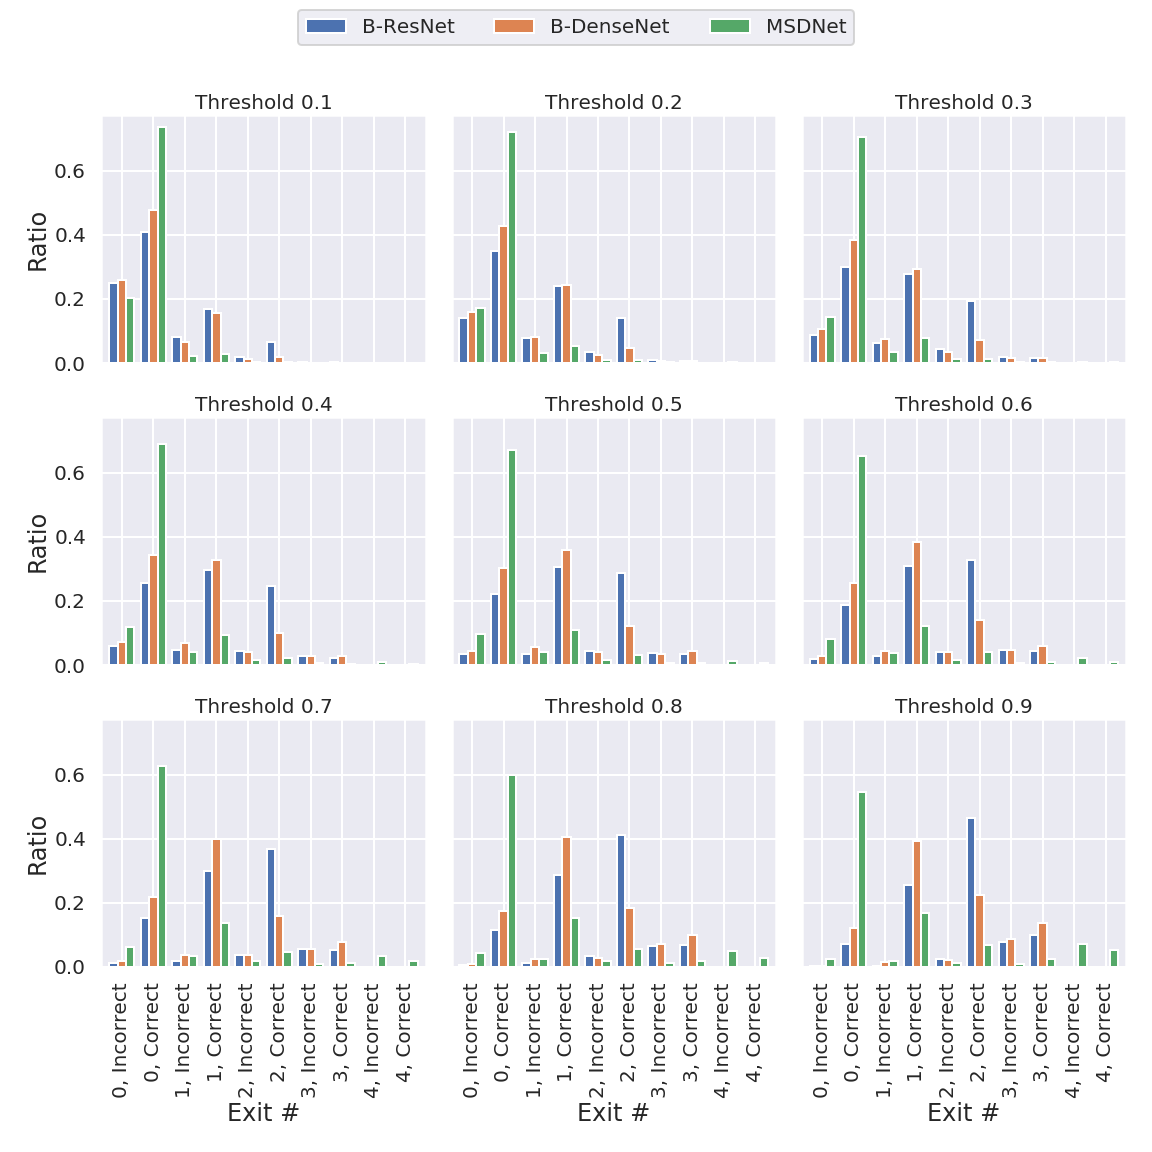
\includegraphics[width=\linewidth]{figures/threshold_plots/inference_threshold_test}
	\caption{Score-Margin Exiting}
	\label{fig:inferencethresholdtest}
\end{figure}

Conventional versions of the \gls{resnet} and \gls{densenet} were trained on the \gls{min100}. Transfer learning was used with ImageNet weights, the model are used as a feature extractor, hence all weights were frozen and only the linear classifier was trained. The conventional models were used to compare with early exiting inference accuracy and latency on X different platforms.

The model inference characteristic on PC, see figure \ref{fig:early_exit_vs_conv}.

  \begin{figure}
  	\captionsetup[subfigure]{justification=centering}
  	\centering
  	\subfloat[Window PC\label{fig:early_exit_vs_conv}]{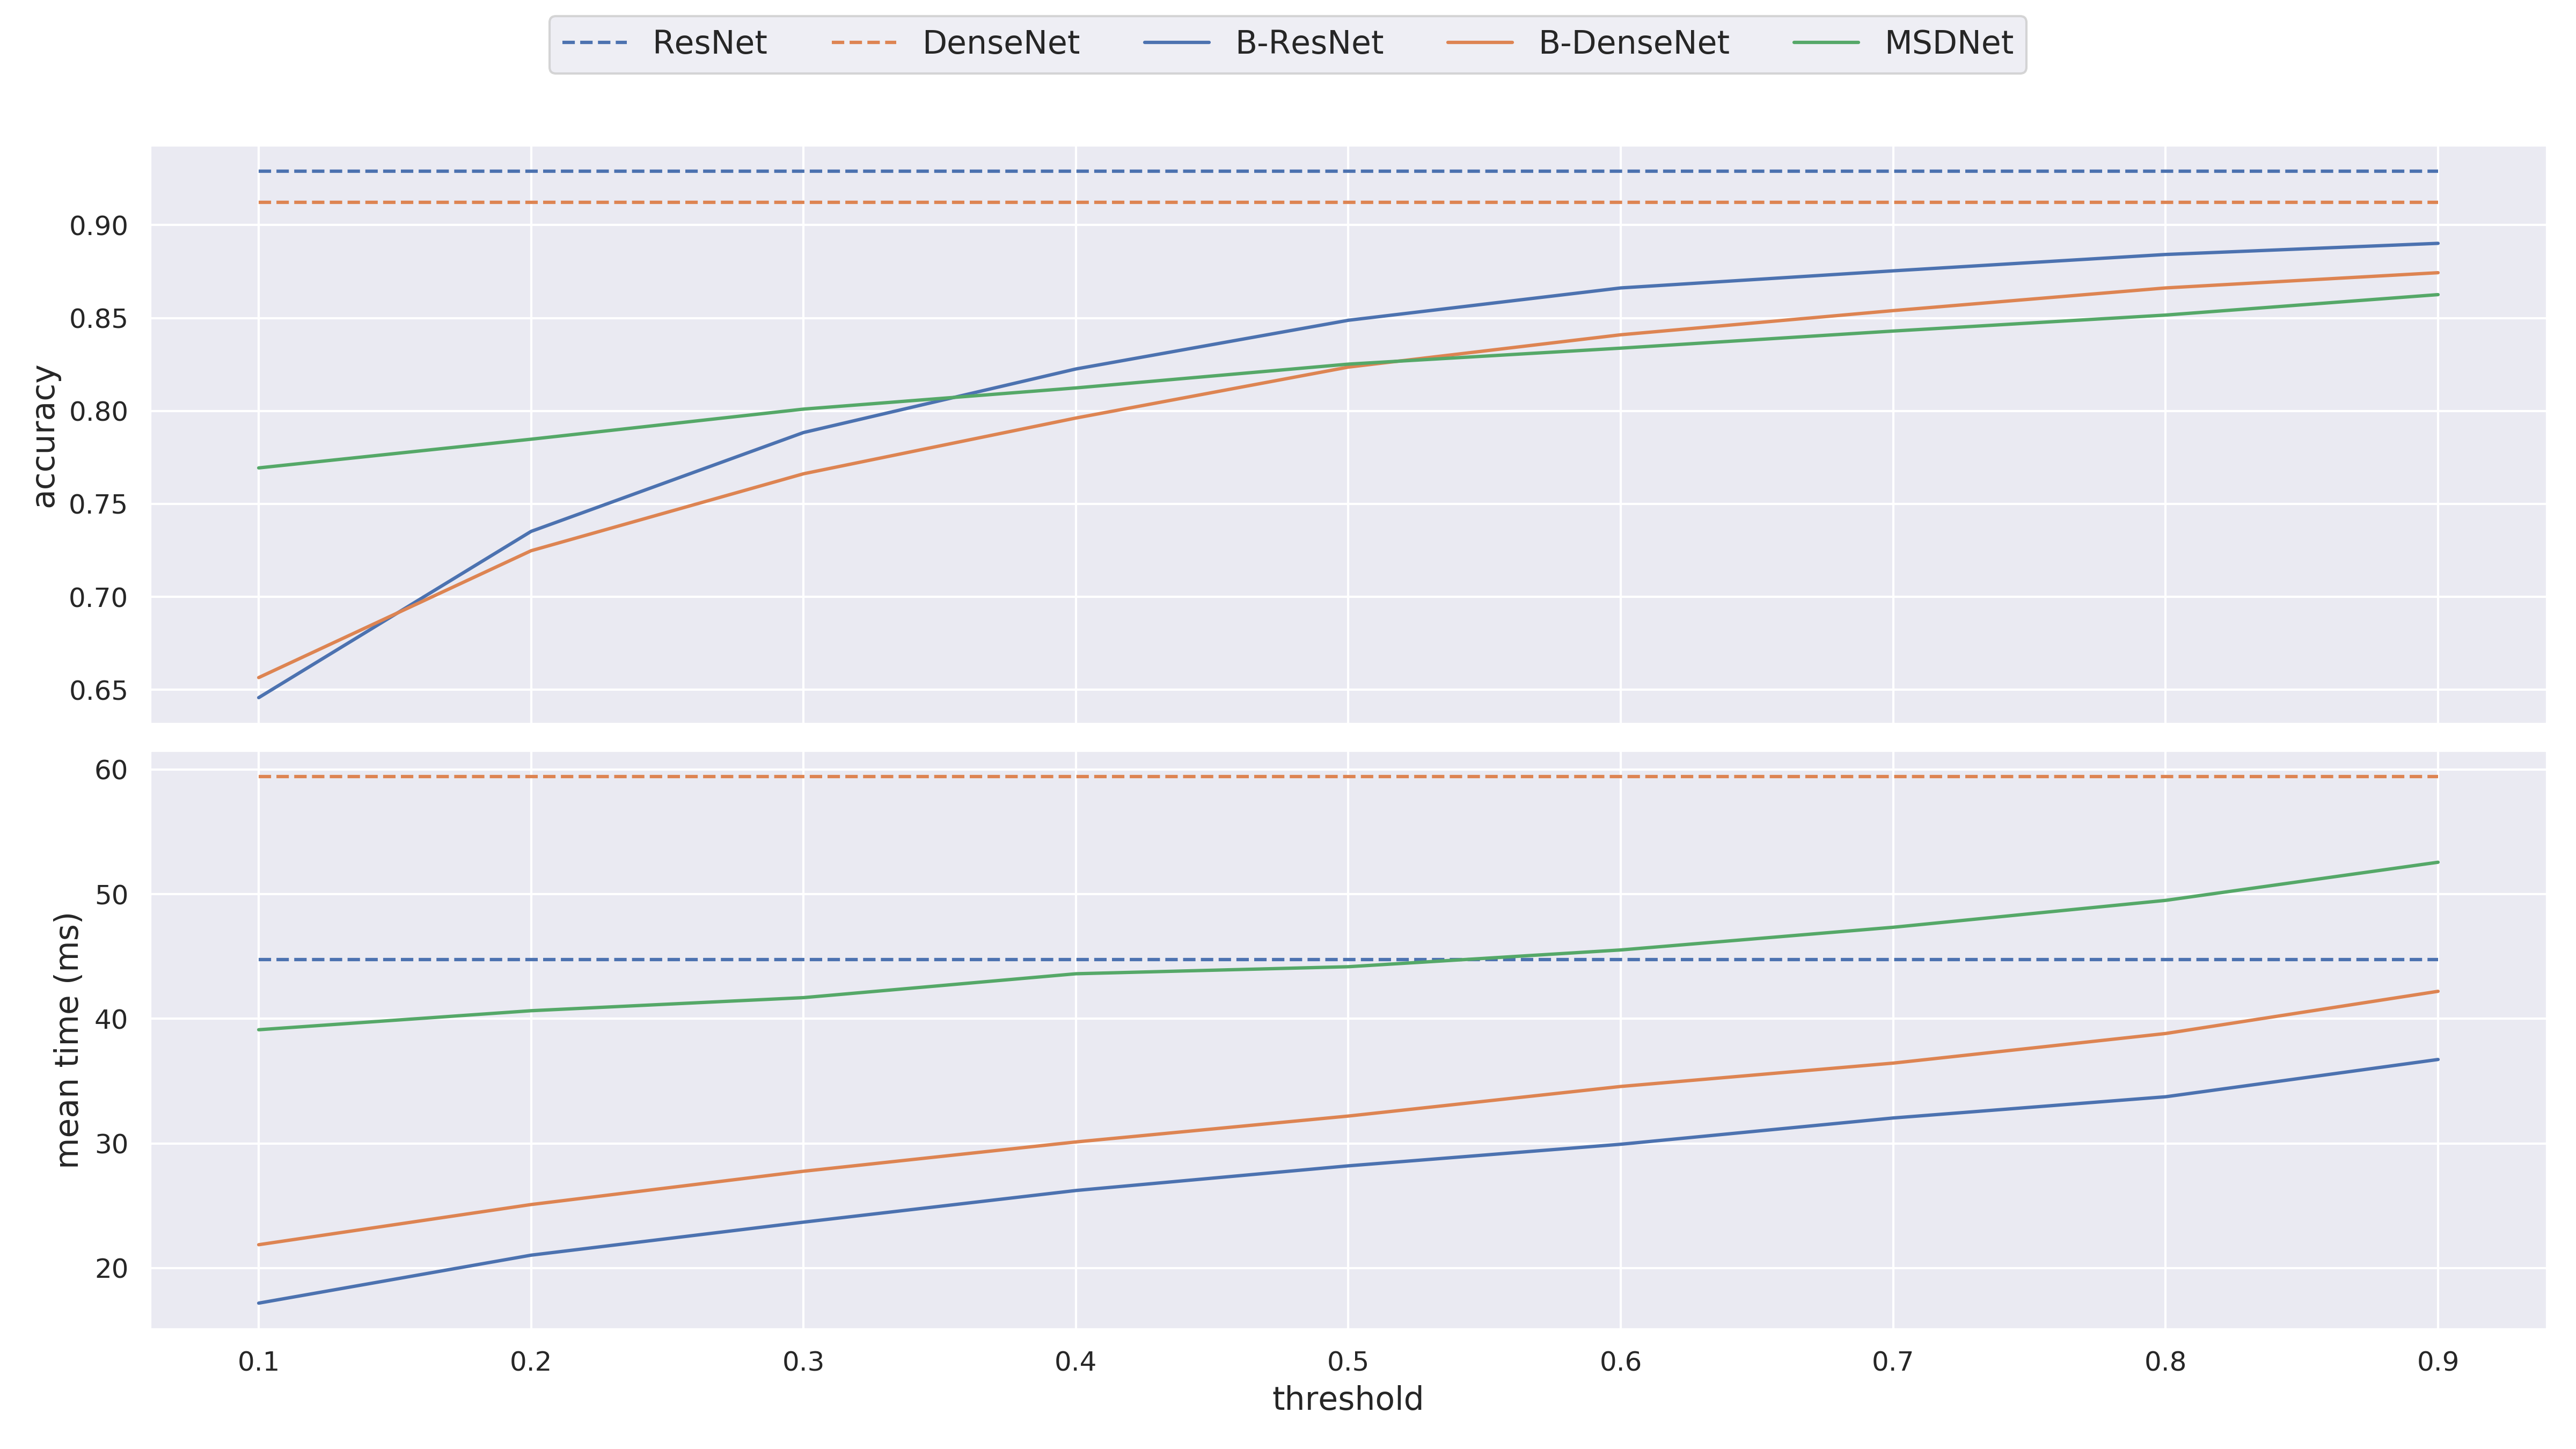
\includegraphics[width=\textwidth,height=.29\textheight,keepaspectratio]{figures/threshold_plots/compare_exiting_vs_no_exiting}}
  	\hfill
	\subfloat[Jetson TX2\label{fig:jetson-early_exit_vs_conv}]{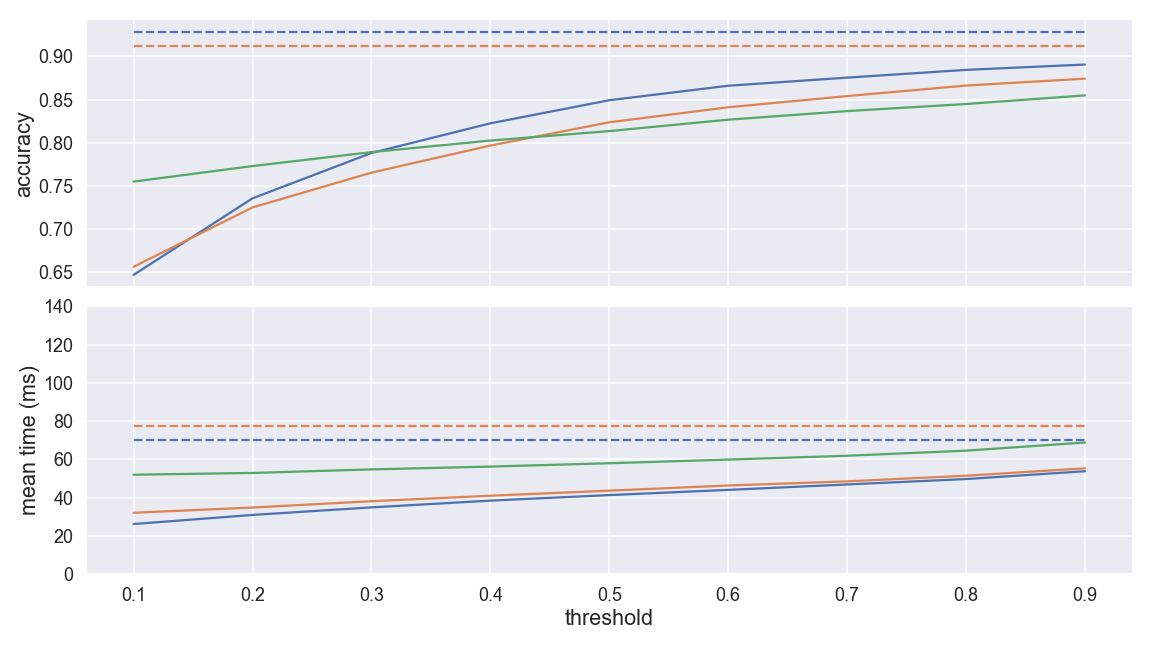
\includegraphics[width=\textwidth,height=.29\textheight,keepaspectratio]{figures/threshold_plots/jetson_inference}}
	\hfill
	\subfloat[NUC\label{fig:nuc-early_exit_vs_conv}]{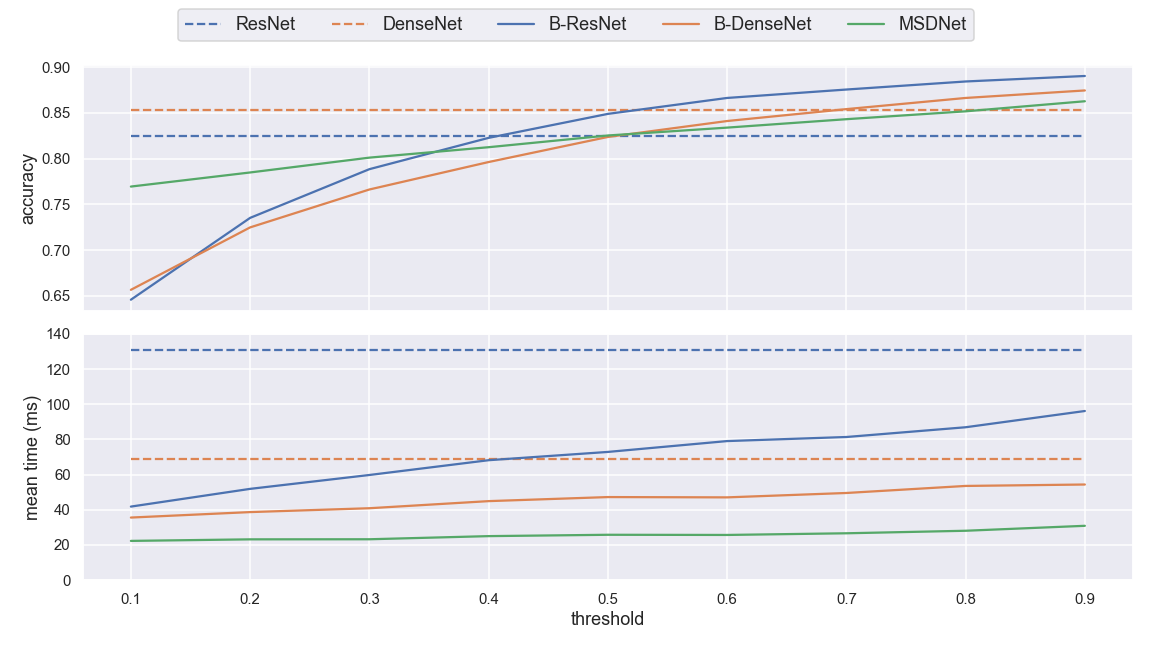
\includegraphics[width=\textwidth,height=.29\textheight,keepaspectratio]{figures/threshold_plots/nuc_inference}}
	\caption[short text]{text}
\end{figure}

The figure clearly states the accuracy-latency trade-off imposed by early exiting. The conventional models are clearly more accurate, however also expectantly slower, than their more flexible exiting counterpart. B-\gls{densenet} benefits more from early exiting, when a threshold of 0.9 is chosen, it gives up 4 percentage point in accuracy and reducing inference latency by 29 \%. The B-\gls{resnet} have about the same compromise in terms of accuracy, however only a reduction of 18 \% inference latency. B-\gls{resnet} still perform better in terms of both accuracy and inference time. The \gls{resnet}. 

  \begin{figure}
	\captionsetup[subfigure]{justification=centering}
	\centering
	\subfloat[Jetson TX2 fine-grained\label{fig:jetson-fingrained}]{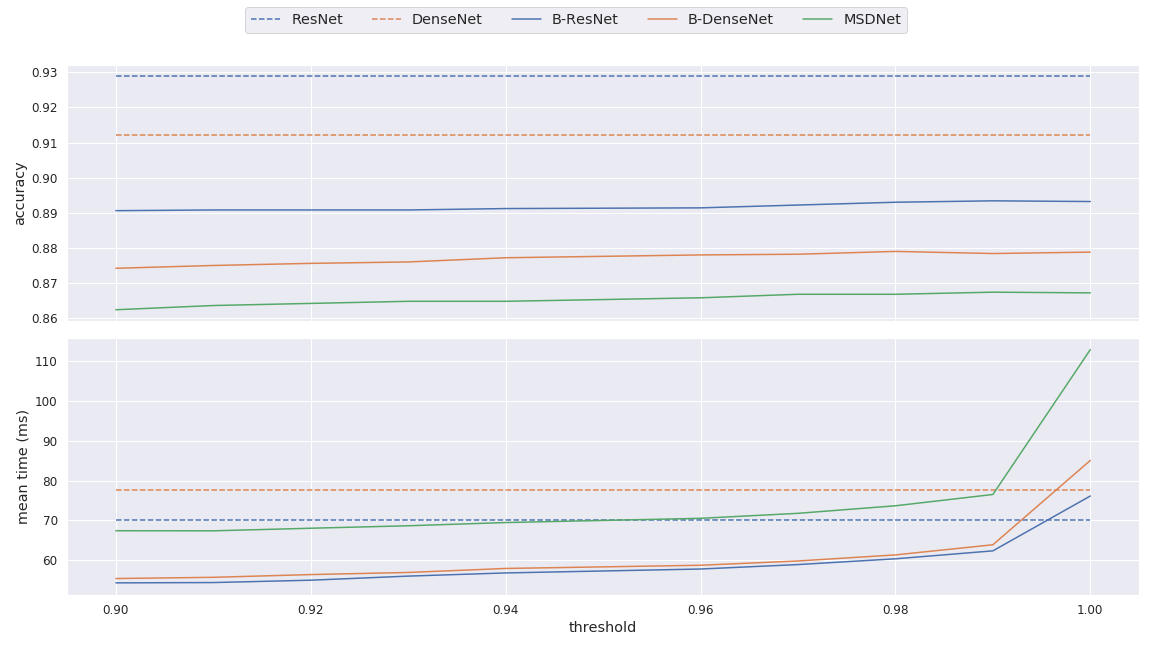
\includegraphics[width=\linewidth]{figures/threshold_plots/jetson_inference_finegrained}}
	\caption[]{}
\end{figure}

\subsection{Delay Threshold Analysis}

For time-budgeted applications, where a classification must be derived within a timed threshold. We wish to maximize the accuracy subject to this time constraint. Figure \ref{fig:time-threshold} show the model accuracy under different time constraints and on different platforms.

How to choose threshold?
If given a time threshold, what accuracy are we then able to achieve? 

\begin{figure}
	\captionsetup[subfigure]{justification=centering}
	\centering
	\subfloat[GPU Workstation]{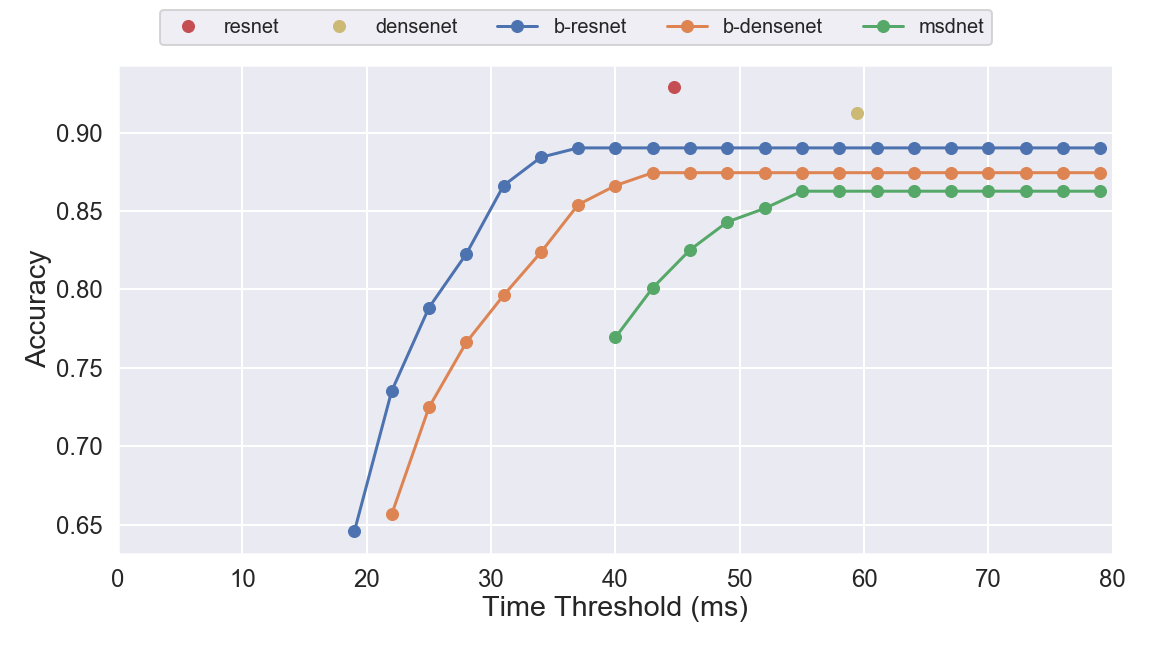
\includegraphics[width=\textwidth,height=.29\textheight,keepaspectratio]{figures/threshold_plots/time_threshold_pc}}
	\hfill
	\subfloat[Jetson TX2]{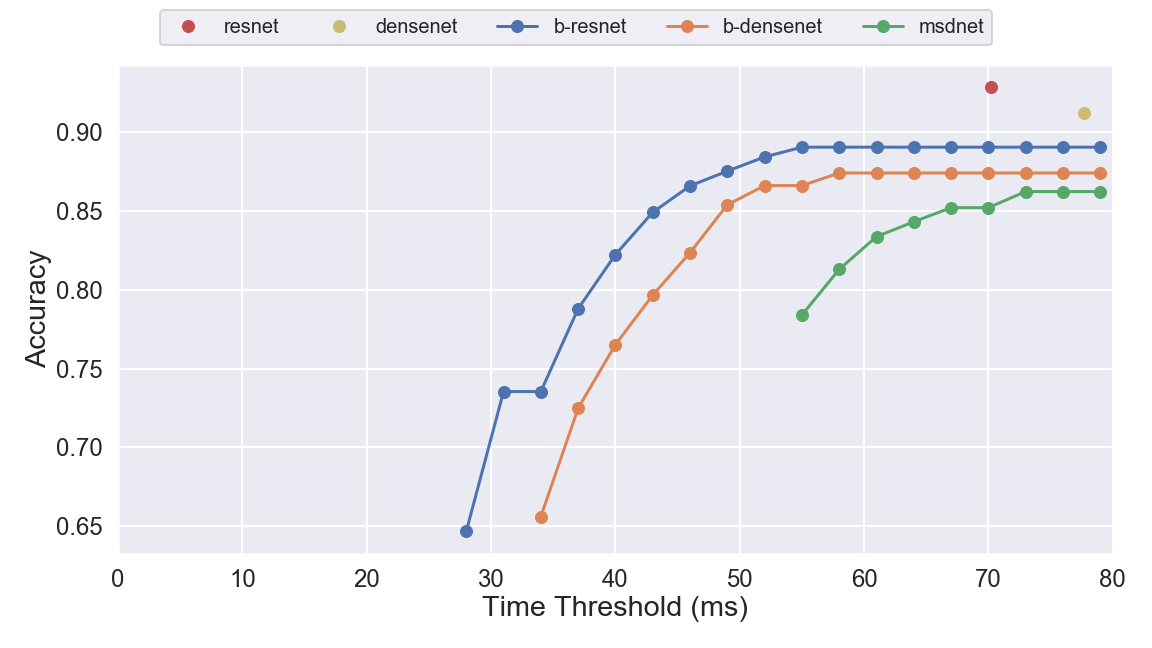
\includegraphics[width=\textwidth,height=.29\textheight,keepaspectratio]{figures/threshold_plots/time_threshold_jetson}}
	\hfill
	\subfloat[NUC]{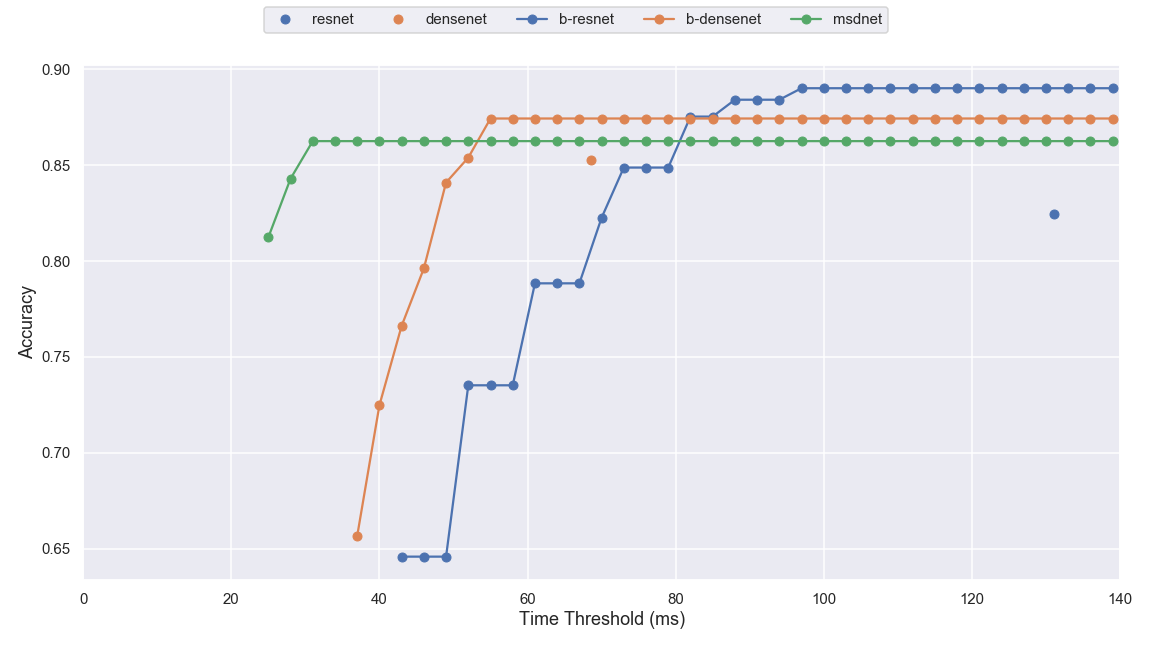
\includegraphics[width=\textwidth,height=.29\textheight,keepaspectratio]{figures/threshold_plots/time_threshold_nuc}}
	\caption[Time Threshold]{Time Threshold}
	\label{fig:time-threshold}
\end{figure}

From figure \ref{fig:inference-time-dist} we know the inference time distribution for each exit on different hardwares. Given a time constraint, we can selective choose the exit with the best chance to provide a prediction within a certain time frame, similar to Edgent \cite{li_edge_2018}. The difference at first is we only focus on on-device or on-edge execution  with no collaboration, hence we do not need a regression model of the per layer execution of the \gls{dnn}. For device-only execution our only concern is the inference time on the specific hardware, a simple selection would be the exit with the largest inference time mean within the time constraint, as accuracy is monotically increasing over available time.
\begin{maxi*}
			{}{Reliabilty\sim\tau_{computation}}
	{}{}
	\addConstraint{\tau_{computation}}{\leq T}
\end{maxi*}
 In an edge-offloading scenario we must consider communication latency. If the available networking conditions are good a later exit can be chosen to improve the reliability, however in scenarios, where networking conditions are poor an earlier exit must be chosen to meet latency requirements. 
 \begin{maxi*}
 	{}{Reliabilty\sim\tau_{computation}}
 	{}{}
 	\addConstraint{(\tau_{computation}+\tau_{communication})}{\leq T}
 \end{maxi*}
The selection of exit is based on distributions of inference time, this introduces some uncertainty, as not all samples might be able to meet the latency requirement, this can be caused be derivation in compute time, congestions in the network latency or server workload. One key feature of early exiting is the ability to obtain intermediate predictions, this allow for parallel execution while offloading. The end-device might only be able to reach an early exit within the time frame, where edge server reaches a later one. However, unexpectedly no reply is received by the end-device within the time frame, then the application can use the local obtained prediction from an earlier exit. 

Or a collaborative scheme might be used, where the end-device locally processes the algorithm up to an early exit and obtains a prediction, then it offload the rest of the execution in a cascaded manner for remote execution, still if no reply is received by the end-device within the time frame a locally obtained prediction is available albeit less reliable than if the remote prediction would have arrived in time. Multiple early exits allows for successively sending back increasingly confident and reliable predictions, at a small overhead communication, the last received prediction would then be used by the application.